\documentclass{article}

% Double-blind main-track submission.
\usepackage[preprint]{neurips_2026}

\usepackage[utf8]{inputenc}
\usepackage[T1]{fontenc}
\usepackage{hyperref}
\usepackage{url}
\usepackage{booktabs}
\usepackage{amsfonts}
\usepackage{amsmath}
\usepackage{graphicx}
\usepackage{xcolor}
\usepackage{microtype}
\usepackage{multirow}
\usepackage{placeins}  % \FloatBarrier to keep figures with their text

% Loosen LaTeX float placement: allow figures to take more of a page
% and require less text per page so figures don't all defer to the end.
\renewcommand{\topfraction}{0.92}
\renewcommand{\bottomfraction}{0.92}
\renewcommand{\textfraction}{0.05}
\renewcommand{\floatpagefraction}{0.7}
\setcounter{topnumber}{3}
\setcounter{bottomnumber}{2}
\setcounter{totalnumber}{4}

% Visible placeholder macro for numbers pending experiment completion.
% Final submission: audit \TODO and replace each with real values.
\newcommand{\TODO}[1]{\textcolor{red}{\textbf{[TODO: #1]}}}

\title{How Foveated Vision Shapes Cognitive Maps in Navigation Agents}

\author{%
  Anonymous authors\\
  Paper under double-blind review\\
}

\begin{document}
\maketitle

\begin{abstract}
What shapes the content of a recurrent navigation agent's learned internal state --- the task, the architecture, or the structure of the visual input? Prior work has shown that blind PointNav agents spontaneously develop cognitive-map-like representations in their recurrent state under task pressure alone~\citep{wijmans2023emergence}. We show that the blind result is a special case of a broader principle: \emph{the visual encoder's information capacity determines whether the LSTM has to carry world-frame spatial structure}. Holding task, optimiser, and LSTM backbone identical and varying only the visual pathway (no vision; a resolution-collapsed encoder; uniform vision; foveated vision at a fixed gaze; foveated vision with a learned gaze), we probe the recurrent state for world-frame position and heading. All five conditions encode top-layer GPS in their LSTM in the typical-episode window. What separates conditions is what happens \emph{later}: when the encoder hands the LSTM minimal spatial-feature variety per step (blind: no encoder; matched-compute: $1{\times}1$ feature map), the LSTM \emph{maintains} a persistent, integration-capable code across episode duration; when the encoder hands it richer spatial features (full-resolution encoders, $8{\times}8$ feature map), the LSTM \emph{overwrites} the GPS code as those visual features take over. We call this the \emph{encoder--memory race}; it recasts the ``cognitive maps emerge without vision'' story as ``cognitive maps emerge — and persist — when the visual pathway cannot resolve the map on its own.'' A second finding cuts across conditions: five agents that solve the task equally well develop recurrent representations in essentially orthogonal linear subspaces, and cross-condition memory transplants incur task cost well above transplant mechanics --- sensor structure shapes representational \emph{format}, not only strength. A third question --- whether static gaze location within a rich-encoder regime acts as a second content axis --- is tested by a foveated-shifted causal control whose training is in progress. The H1 ordering reproduces on a held-out MP3D evaluation, consistent with an agent-internal rather than Gibson-specific mechanism. Three implications, each scoped to the recurrent PointNav setting we study. \textbf{(i)}~Encoder capacity correlates inversely with linear, top-layer LSTM spatial encoding; \emph{if} the correlation reflects causation (which the encoder-resolution scaling sweep, in progress, tests directly), it would also be a practical training-time lever for inducing cognitive-map-like internal representations. \textbf{(ii)}~``More pixels, richer memory'' is the wrong intuition within this setup; the relationship across our five conditions is inverse. \textbf{(iii)}~The pattern parallels independent animal-navigation findings --- enhanced hippocampal coupling in congenitally blind humans, the disruption of rodent grid-cell firing in the dark (with navigation nonetheless preserved), cross-modality hippocampal remapping in bats --- without depending on their biophysics, suggestive of a sensor--memory coupling principle whose generality across architectures (transformers, non-RL learners, non-navigation tasks) we do not test here.
\end{abstract}


\section{Introduction}

Primate spatial memory is shaped by how primates see. Hippocampal cells code joint place--view--action state precisely because primates sample the scene through a foveated sensor that resolves a small high-acuity region per glance~\citep{wirth2017gaze,rolls2024why}; rodents with near-panoramic vision instead show classic place fields. Sensor structure also reorganises memory \emph{within} a single animal: bats produce non-overlapping hippocampal populations when they switch between vision and echolocation~\citep{geva2016remapping}; congenitally blind humans develop enhanced hippocampal coupling and outperform sighted controls on non-visual spatial tasks~\citep{kupers2014blind}. The biological pattern is consistent: \emph{the structure of the sensor reshapes the structure of spatial memory}. We ask whether the same is true of artificial navigation agents.

The recent emergent-cognitive-maps literature has shown that navigation agents trained with deep RL spontaneously develop spatial representations in their recurrent state, even without visual input~\citep{wijmans2023emergence}, and that grid-cell-like structure can emerge in path-integration networks~\citep{banino2018grid,cueva2018grid}. These results establish that \emph{some} map-like structure is learned without being designed in. They leave open the complementary question we take up here: holding task and architecture fixed, does the structure of the visual sensor reshape \emph{what} recurrent memory encodes --- and if so, how? We test this by training otherwise-identical DD-PPO PointNav agents under five visual sensor conditions: \emph{blind} (no vision), \emph{uniform} (full $256{\times}256$ RGB), \emph{foveated} with a fixed central gaze, \emph{foveated with a learned gaze}, and a \emph{matched-compute} control that down-samples the input until the encoder's spatial output collapses to a single feature vector. The matched-compute condition is included to separate ``no vision'' from ``vision the encoder cannot resolve'': it has visual input, but its $1{\times}1$ encoder feature map provides minimal spatial structure to the LSTM. The five conditions span a sensor-structure spectrum on which foveation occupies a biologically motivated point.

\begin{figure}[!htbp]
\centering
\begin{minipage}{\linewidth}\centering
\begin{minipage}{0.30\linewidth}\centering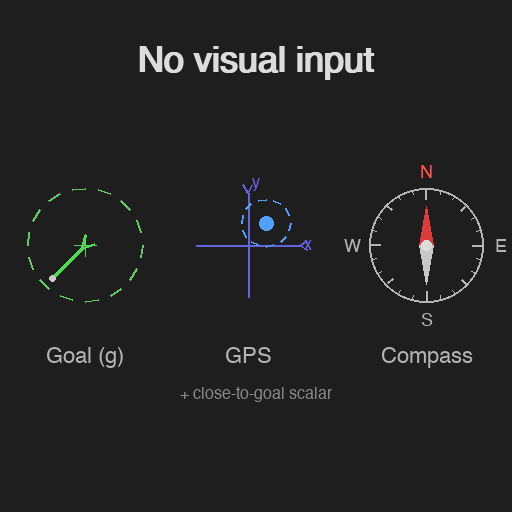
\includegraphics[width=\linewidth]{fig/fig_blind.png}\\{\footnotesize (a) Blind}\end{minipage}\hfill
\begin{minipage}{0.30\linewidth}\centering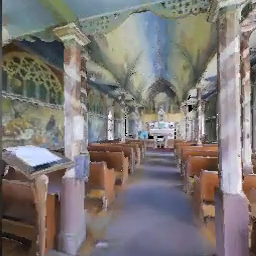
\includegraphics[width=\linewidth]{fig/fig_uniform.png}\\{\footnotesize (b) Uniform}\end{minipage}\hfill
\begin{minipage}{0.30\linewidth}\centering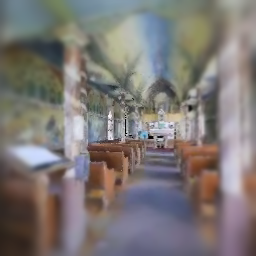
\includegraphics[width=\linewidth]{fig/fig_foveated.png}\\{\footnotesize (c) Foveated (fixed gaze)}\end{minipage}\\[6pt]
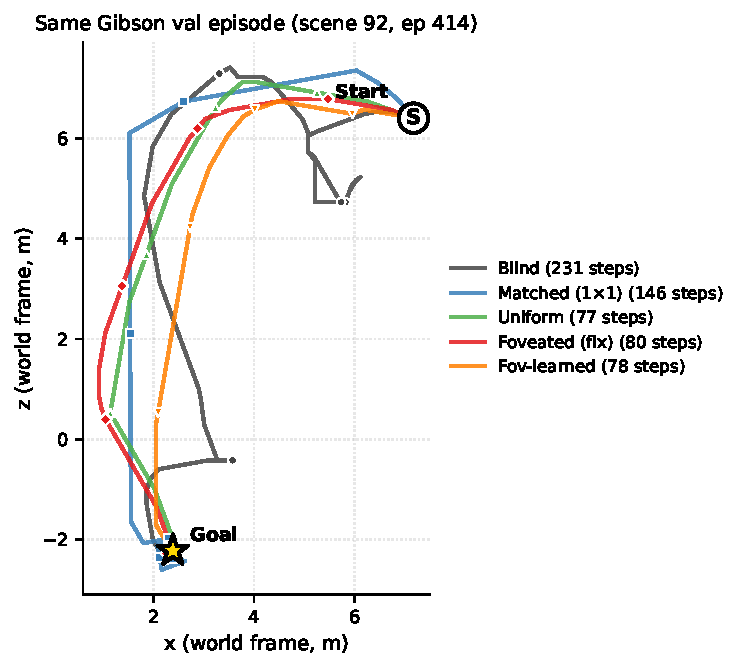
\includegraphics[width=0.95\linewidth]{fig/trajectory_overlay.pdf}\\[2pt]
{\footnotesize (d) The 5 conditions on the same MP3D-train episode (scene E9uDoFAP3SH, ep 40422 in the env iterator; same paired index 414 across our probing data), trajectories overlaid on the Habitat-rendered top-down occupancy map. Each condition's SPL on this episode is within $\pm 0.10$ of its per-condition median, so all five are typical successful runs. Bottleneck conditions (blind 231 steps, matched 146) take longer paths through the corridor; rich-encoder conditions (uniform / foveated / fov-learned, 77--80 steps) take near-direct paths along the same corridor.}
\end{minipage}
\caption{The five visual conditions differ only in what reaches the agent's encoder, but produce visibly different navigation behaviours. \emph{Inputs:} (a) Blind: no visual input; only the non-visual sensor stack (goal-in-start-frame, GPS, compass, close-to-goal scalar) --- the Wijmans~\citep{wijmans2023emergence} configuration. (b) Uniform: $256\times 256$ full-resolution RGB. (c) Foveated (fixed gaze): eccentricity-dependent Gaussian blur centred on the image middle ($\sigma_{\max}=8$, quadratic falloff). Two additional conditions not pictured: \emph{matched-compute} (a down-sampled uniform view at $48\times 48$, whose total pixel budget matches foveated and whose ResNet-18 encoder produces a $1{\times}1$ feature map) and \emph{foveated (learned gaze)}, which adds a learned $(x,y)$ gaze offset to (c). \emph{Behaviour:} (d) all five conditions solve the same PointGoal navigation task; the trajectory shape and length differ systematically, previewing the encoder--memory race finding (§\ref{sec:h1}).}
\label{fig:setup}
\end{figure}

All conditions share an identical DD-PPO learner, the same Gibson-0$+$MP3D training pool, the same LSTM backbone, and the same non-visual sensor stack (goal-in-start-frame, GPS, compass, close-to-goal scalar; Figure~\ref{fig:setup}); they differ only in what reaches the visual encoder. We test three hypotheses. \emph{H1 (encoder--memory race)}: when the visual encoder supplies the LSTM with little spatial-feature variety per step, the recurrent state should compensate by maintaining a world-frame spatial code; richer encoder output should let the LSTM rely on visual features instead. \emph{H2 (sensor structure $\to$ format divergence)}: different sensor conditions should produce hidden-state representations in distinct linear subspaces, not scaled versions of a common code. \emph{H3 (gaze location $\to$ orthogonal content lever)}: within the rich-encoder regime, where a foveated sensor is centred should act as a content axis independent of the sensor transform. Each hypothesis has a direct biological analog --- compensatory hippocampal coupling under reduced sensory access~\citep{kupers2014blind,chen2016grid}; cross-modality remapping in single animals~\citep{geva2016remapping}; the saccade-gated hippocampal theta whose reliability predicts memory~\citep{jutras2013saccades,tas2016overt} --- which we use as convergent (not conclusive) evidence and discuss in §\ref{sec:bio}.

The empirical findings, in order of evidence strength. \emph{(i) An encoder--memory race emerges along the sensor-structure spectrum.} All five conditions encode top-layer GPS in the typical-episode window, but only conditions with minimal encoder spatial output --- blind (no encoder) and matched-compute ($1{\times}1$ encoder feature map) --- \emph{maintain} the code across episode duration; rich-encoder conditions (uniform, foveated, foveated-learned) overwrite it as visual features accumulate. Direct probing of the encoder output sharpens the mechanism: no sighted encoder linearly decodes world-frame GPS, so the H1 divergence is not about encoder-level position retention. It is about how much spatial-feature variety the encoder supplies, and whether that variety is enough to substitute for integrating the LSTM's sensor-branch GPS input across time. The pattern is preserved on a held-out MP3D evaluation. \emph{(ii) Sensor structure shapes representational format.} Even agents that solve the same task at the same success rate develop hidden states in essentially disjoint linear subspaces (pairwise CKA $<10^{-4}$, $1$-NN purity $1.000$, cross-condition probe transfer that predicts off-manifold values), and cross-condition memory transplants between rich-encoder pairs degrade task performance well beyond same-condition mechanics. The transplant matrix is asymmetric: bottleneck-condition hidden states hurt rich-encoder recipients far more than vice versa. \emph{(iii) Foveation specifically diverges from uniform on H2 / behaviour / dataset shift, even where the H1 readout is similar.} Under our $\sigma_{\max}=8$ Gaussian-blur foveation model, foveated and uniform agents agree on top-layer GPS $R^2$ but differ on cross-condition transplant compatibility, behavioural memory reliance (shortcut SPL drop), and held-out MP3D recovery; whatever foveation does differently from uniform, it does so inside the LSTM in subspaces invisible to a linear-GPS probe. \emph{(iv) Probe-readable and policy-used memory can dissociate.} Plotting probe-readable GPS against behavioural memory reliance reveals a $2{\times}2$ pattern with two opposite anomalies: matched-compute has a linear top-layer cognitive map but its policy weights it less than the probe predicts, and uniform has no linear GPS yet relies heavily on memory --- plausibly via non-spatial scene-history features. \emph{(v) H3 (gaze location)} is tested by a foveated-shifted causal control whose training is in progress at submission.

We position these as five connected statements about how visual sensor structure reshapes recurrent memory in a controlled agent setting. Each has a direct biological precedent (§\ref{sec:bio}). The findings are correlation-level over our five conditions; an encoder-resolution scaling sweep that varies input size at fixed encoder stack is in progress and would test the H1 mechanism causally (Appendix~\ref{app:scaling}). The most striking foveation-specific predictions --- that spatial-sampling foveation (log-polar) should trigger the encoder--memory race in a way that soft Gaussian blur does not --- depend on experiments still in training; we disclose them as falsifiable predictions in §\ref{sec:foveation} and Appendix~\ref{app:foveation-status}.


\section{Related Work}

\noindent\textbf{Cognitive maps in RL navigation agents}\quad Wijmans et al.~\citep{wijmans2023emergence} demonstrated that map-like representations emerge in the recurrent memories of DD-PPO agents even without visual input; Dwivedi et al.~\citep{dwivedi2022isee} probed sighted agents for related spatial concepts; Banino et al.~\citep{banino2018grid} and Cueva \& Wei~\citep{cueva2018grid} found grid-cell-like units in recurrent networks trained on path integration; Gornet \& Thomson~\citep{gornet2024cognitive} extended this via visual predictive coding. Hennig et al.~\citep{hennig2023belief} showed that RL under partial observability can induce belief-state-like representations without explicit probabilistic objectives. Ramakrishnan et al.~\citep{ramakrishnan2025space} examined spatial cognition in frontier models. All these studies use either absent or spatially uniform perception; none vary input quality spatially, and none test whether different sensors produce different representational formats.

\noindent\textbf{Foveated vision and gaze policies in deep learning}\quad Foveated rendering~\citep{strasburger2011peripheral,rosenholtz2016peripheral} exploits eccentricity-dependent acuity falloff for efficiency. Learned glimpse policies appear in recurrent attention models~\citep{mnih2014attention}; Atanov et al.~\citep{atanov2024photoreceptor} showed that sensor layout changes downstream task performance. Pourrahimi \& Bashivan~\citep{pourrahimi2025foveated} probed a foveated visual-search model for neuroscience-predicted features; Shang \& Ryoo~\citep{shang2023sugarl} jointly learned gaze and motor policies following the Sprague \& Ballard~\citep{sprague2003eyemovements} framework. These address visual search or task performance; none asks how sensor structure reshapes the learned spatial memory of a downstream navigation policy.

\noindent\textbf{Probing neural representations}\quad Belinkov~\citep{belinkov2022probing} surveys probing classifiers; Hewitt \& Liang~\citep{hewitt2019control} introduced control tasks to distinguish genuine structure from probe memorisation; Kornblith et al.~\citep{kornblith2019cka} introduced linear CKA for cross-model similarity. We adopt linear probing, the Hewitt--Liang selectivity metric, and unaligned linear CKA, and complement them with two behavioural interventions directly on the recurrent state (memory transplant and shortcut discovery) to validate the probe-based findings outside the linear-probe framework.

\noindent\textbf{Biological precedent}\quad Our hypotheses and framing draw on three threads of animal-navigation research. (i)~Primate hippocampal cells code joint place--view--action state~\citep{wirth2017gaze,rolls2023viewcells}; Rolls~\citep{rolls2024why} argues that primate \emph{spatial-view cells} and rodent \emph{place cells} reflect the different sampling statistics of foveated versus near-panoramic vision. (ii)~The same bat in the same environment produces non-overlapping hippocampal populations when it switches between vision and echolocation~\citep{geva2016remapping}---format-level divergence across sensor modalities within a single animal. (iii)~In primates, each saccade resets hippocampal 3--8 Hz rhythms and the reliability of the reset predicts subsequent memory~\citep{jutras2013saccades}; only overt (not covert) attention automatically writes to visual working memory~\citep{tas2016overt}. Gaze targets themselves are selected in an information-gain-maximising fashion consistent with ideal-observer predictions~\citep{najemnik2005optimal,gottlieb2013information,hayhoe2018control}. We use these results only to frame our ML predictions and interpret our findings; our contribution is the controlled ablation in a learned agent that cross-species and cross-modality biological comparisons cannot cleanly supply.

\noindent\textbf{What is new here}\quad Three things distinguish this work from the studies above. (i)~A \emph{controlled} five-condition ablation with everything but the visual pathway held identical, including the matched-compute condition that decouples ``no vision'' from ``visual encoder bottleneck'' --- the lever that makes the encoder--memory race claim falsifiable. (ii)~A protocol-corrected probing methodology: deterministic action selection at probe time (the policy used by every other component of our eval pipeline) rather than stochastic sampling, which we found inflates probe $R^2$ for high-entropy policies via a 4-step quasi-static-trajectory artefact (§\ref{sec:methods-probes} and Appendix~\ref{app:probing-details}). (iii)~Convergent behavioural validation of the probe-based H1 and H2 findings via memory transplant and shortcut discovery, both of which sit \emph{outside} the linear-probe framework.


\section{Methods}

\subsection{Setup}
\label{sec:methods-setup}

All agents are trained on PointGoal navigation in Habitat~\citep{savva2019habitat} using DD-PPO~\citep{wijmans2020ddppo} on a merged pool of Gibson-0+~\citep{xia2018gibson} (411 scenes) and Matterport3D train (61 scenes), totalling 472 training scenes; evaluation uses 18 held-out MP3D test scenes (1008 episodes). All agents share an identical 3-layer LSTM (512-d) backbone and the Wijmans non-visual sensor stack (goal-in-start-frame, GPS, compass, close-to-goal scalar), each projected to 32-d and concatenated with a 32-d previous-action embedding. All sighted conditions train to $\sim$250M environment frames; the blind baseline trains to 342M to allow slower convergence from proprioception alone.

The five visual conditions (Figure~\ref{fig:setup}): \emph{blind} (no visual input); \emph{uniform} (full $256{\times}256$ RGB encoded by ResNet-18); \emph{foveated (fixed)} (eccentricity-dependent Gaussian blur, $\sigma_{\max}=8$ quadratic falloff, gaze locked at image centre, same ResNet-18 encoder); \emph{matched-compute} ($48{\times}48$ uniform RGB; at this resolution ResNet-18's 32-fold spatial downsampling collapses the feature map to $1{\times}1$, removing spatial structure but preserving channel information); \emph{foveated (learned)} (same blur model, gaze centre predicted by a lightweight MLP trained end-to-end). Matched-compute is the spatial-bandwidth lower bound for our encoder; it has visual input but its encoder output cannot resolve world-frame position. The $48{\times}48$ input also has lower spatial resolution than uniform's $256{\times}256$, so this single condition cannot fully separate the $1{\times}1$ collapse from low input resolution; the encoder-resolution scaling sweep (Appendix~\ref{app:scaling}) addresses this directly. The foveated conditions disable the running-mean-and-variance input normaliser to avoid an in-place autograd conflict along the gaze-decoder gradient path; an invariance control is in training. We also discovered and patched a silent NaN-gradient corruption mode in DD-PPO (Appendix~\ref{app:training-stability}).

\subsection{Probes}
\label{sec:methods-probes}

After training, all weights are frozen. We collect per-step top-layer LSTM hidden states ($512$-d) paired with ground-truth labels from $n{=}500$ Gibson held-out episodes under \emph{deterministic} argmax-action rollouts (matching our shortcut / transplant / standard eval protocols; the alternative stochastic protocol gives trivial $\sim 4$-step rollouts and is documented in Appendix~\ref{app:probing-details}). We train Ridge probes ($\alpha=10$) with episode-level 5-fold cross-validation, report mean $\pm \sigma$ across folds, and verify probe specificity with Hewitt--Liang label-permutation selectivity~\citep{hewitt2019control}. Probed variables: GPS position, compass heading, distance-to-goal, lag-$k$ path history ($k \in \{0, \ldots, 20\}$), visited-region occupancy, full occupancy grid, per-unit spatial information, ego-frame goal vector. For H2 representational geometry we additionally use linear CKA~\citep{kornblith2019cka} and cross-condition probe transfer.

We complement probes with two interventions on the LSTM state. \emph{Memory transplant}: paste a donor's hidden state into the recipient at step $30$ and compare baseline / self-transplant / cross-transplant SPL across $150$ episodes per pair. \emph{Shortcut discovery}: run paired same-scene-different-goal episodes ($20$ scenes $\times$ $10$ pairs) and compare second-episode SPL under reset vs.\ persistent LSTM. For foveated-fixed, all analyses use ckpt.36 at $\sim$174M frames (last clean intermediate before the silent-corruption window).


\section{Results}
\label{sec:results}

\subsection{Five conditions, same task}
\label{sec:summary}

Table~\ref{tab:summary} collects the headline per-condition numbers this section returns to. All sighted conditions solve PointGoal at $96$--$99\%$ success; blind reaches $93\%$ at a longer training budget, reproducing Wijmans et al.~\citep{wijmans2023emergence}. Success is tightly bunched, so ``the agents differ in what they do'' is an unlikely explanation for the encoded-content gap we report (it does not strictly rule it out). The probe machinery itself is calibrated: distance-to-goal decodes robustly across all five conditions ($R^2 \in [0.81, 0.90]$; Appendix~\ref{app:supp_figs} for the companion plot), confirming that Ridge has the capacity to fit high-$R^2$ scalars when the hidden state contains them; and Hewitt--Liang label-permutation selectivity is high in the conditions where the GPS code itself is high (blind GPS / compass selectivity $+0.95 / +0.81$; matched $+0.72 / +0.56$), consistent with a genuine signal rather than label memorisation. Two training-stability caveats are disclosed in full in Appendix~\ref{app:training-stability}: foveated-fixed uses ckpt.36 at $\sim$174M frames (last clean checkpoint before a silent NaN-gradient corruption at $\approx\!182$M); and matched-compute's $1{\times}1$ feature-map collapse, originally noticed as a training quirk, is what makes matched-compute a useful test of the encoder-bottleneck framing (we cannot from one condition alone fully separate the $1{\times}1$ feature-map effect from the lower input resolution; see §\ref{sec:methods-setup} and §\ref{sec:foveation}).

\begin{table}[!htbp]
\centering
\small
\setlength{\tabcolsep}{6pt}
\caption{Per-condition headline. Probe $R^2$ columns are the 5-fold episode-level CV mean $\pm$ std on full-length deterministic-rollout trajectories (no per-episode step cap). \emph{GPS} and \emph{Compass} are world-frame. The bottleneck-vs-rich-encoder gap is in temporal \emph{stability} of the code, not its mid-episode existence (Figure~\ref{fig:h1_mega}b): all five conditions decode top-layer GPS at $R^2 \in [0.6, 0.95]$ in the typical-episode window (steps 50--200); the rich-encoder long-tail collapse is what produces the sub-chance numbers below. Bold marks the H1-relevant ordering (blind $>$ matched $\gg$ rich-encoder).}
\label{tab:summary}
\begin{tabular}{lccccc}
\toprule
Condition & Frames & SPL & Success & GPS $R^2$ (no-cap) & Compass $R^2$ (no-cap) \\
\midrule
Blind                 & 342M  & 0.59          & 0.93          & \textbf{$+$0.95$\pm$0.02} & \textbf{$+$0.81$\pm$0.08} \\
Matched-compute       & 250M  & 0.67          & 0.98          & \textbf{$+$0.78$\pm$0.10} & \textbf{$+$0.64$\pm$0.10} \\
Uniform               & 250M  & \textbf{0.85} & \textbf{0.99} & $-$0.31$\pm$0.86          & $+$0.36$\pm$0.23 \\
Foveated (fix)        & 174M  & 0.78          & 0.96          & $+$0.06$\pm$0.88          & $+$0.07$\pm$0.69 \\
Fov-learned           & 250M  & 0.82          & 0.98          & $-$2.43$\pm$3.98          & $-$1.34$\pm$3.14 \\
\bottomrule
\end{tabular}
\end{table}


\subsection{Encoder--memory race: a temporal-stability claim (H1)}
\label{sec:h1}

\begin{figure}[!htbp]
\centering
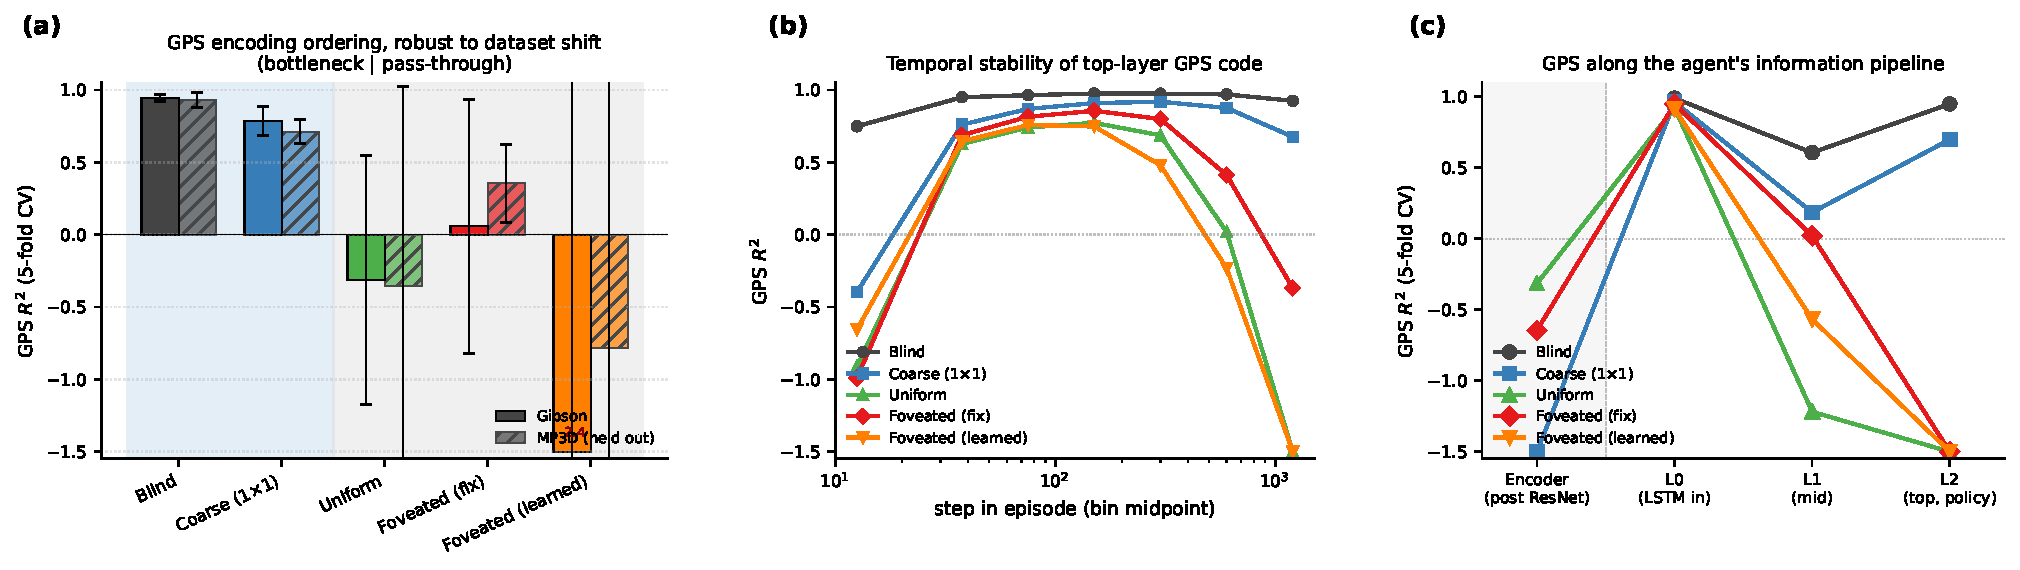
\includegraphics[width=\linewidth]{fig/h1_mega.pdf}
\caption{H1 evidence in three panels. \emph{(a)}~GPS $R^2$ (5-fold CV, Ridge $\alpha=10$, full-length deterministic rollouts) on Gibson and held-out MP3D (300 episodes/condition; same checkpoints, no re-training). Blind and matched-compute (bottleneck conditions, blue background) decode world-frame GPS robustly on both datasets; uniform / foveated / foveated-learned (rich-encoder, grey background) do not, except for foveated recovering to a mild positive ($R^2 = +0.35$) on MP3D. The Compass and DtG numbers are in Table~\ref{tab:summary} (compass shows the same ordering at smaller magnitude; DtG decodes everywhere because every agent must track it; Appendix~\ref{app:supp_figs} for the companion bar plots). \emph{(b)}~Top-layer GPS $R^2$ binned by step-in-episode (out-of-fold prediction): all five conditions encode top-layer GPS in the typical-episode window (steps $\sim 25$--$200$); the rich-encoder conditions then \emph{overwrite} the code (negative $R^2$ in the long-tail $800+$ bin), while bottleneck conditions hold $R^2 > 0.7$ to step $800+$. The headline ``rich-encoder $\approx$ chance'' in panel (a) is therefore primarily long-tail behaviour. \emph{(c)}~Per-LSTM-layer GPS $R^2$ (single-fit on top-layer hidden states): all five conditions have GPS at Layer 0 (where the GPS sensor embedding enters the LSTM input vector --- this lower-bound is at least partly a sensor-pass-through effect, not the network ``computing'' position); the divergence is at Layer~2, the policy readout.}
\label{fig:h1_mega}
\end{figure}

Visual-encoder capacity inversely tracks LSTM spatial encoding across our five conditions: bottleneck conditions (blind, matched) encode GPS / compass at the top layer; rich-encoder conditions (uniform, foveated, foveated-learned) decode at chance (Figure~\ref{fig:h1_mega}a, Table~\ref{tab:summary}). DtG decodes robustly in every condition because every agent must track it. \TODO{Whether the correlation reflects causation is what the §\ref{sec:foveation} experiments and the Appendix~\ref{app:scaling} resolution sweep test; multi-seed gap-fills are in progress.}

\noindent\textbf{Temporal stability is the precise claim}\quad The no-cap probe conflates ``does the LSTM ever encode GPS'' with ``does it maintain the encoding across episode duration.'' Step-binned out-of-fold probing separates them (Figure~\ref{fig:h1_mega}b): all five conditions encode top-layer GPS in the typical-episode window; rich-encoder conditions then \emph{overwrite} the code (chance by step 400--800, deeply negative in the long-tail bin), while bottleneck conditions hold it stable to step 800+. The Table~\ref{tab:summary} ``rich-encoder $\approx$ chance'' headline is therefore long-tail behaviour, not mid-episode. \emph{H1 is most precisely a temporal-stability claim about the linearly-decodable top-layer GPS code.} A lag-$k$ probe corroborates: blind GPS decodes at $R^2 = 0.92$ at $k = 20$, matched $> 0.5$; rich-encoder conditions are at chance for every $k \leq 10$.

\emph{Layer specificity and non-linear probe.} All five conditions have GPS at LSTM Layer 0 because the GPS-sensor embedding enters there (Figure~\ref{fig:h1_mega}c). The H1 distinction is what happens through Layers 1--2: bottleneck retain to Layer 2, rich-encoder discard. Since the DD-PPO action head is a linear projection from $\mathbf{h}_2$, this maps to ``policy-accessible''. A 2-layer MLP on the same top-layer states recovers GPS for rich-encoder conditions ($R^2 \in [0.51, 0.73]$); H1 is therefore precisely about \emph{linear} top-layer decodability, not whether \emph{any} probe can recover position. The MLP result alone cannot exclude exploitation of position-correlated features (wall distance, scene identifiers); Appendix~\ref{app:probe-details} discusses both. The bottleneck-vs-pass-through partition is preserved on held-out MP3D (Figure~\ref{fig:h1_mega}a); two single-seed cross-dataset shifts (foveated GPS chance $\to$ $+0.35$; foveated-learned compass $-1.34 \to +0.41$) await multi-seed replication.

\noindent\textbf{Proposed mechanism}\quad We \emph{propose} the following account, consistent with the data but not directly tested by a causal intervention. In PointNav, GPS and compass enter the LSTM input at Layer~0 directly, via a 32-d sensor embedding concatenated with the visual encoder's flattened output (Figure~\ref{fig:h1_mega}c shows GPS at Layer~0 across all five conditions, $R^2 > 0.91$). The encoder feature-map probe (§\ref{sec:foveation}, Figure~\ref{fig:encoder_probe}) shows that none of the three sighted encoders linearly re-derive GPS from their visual stream: matched $R^2 = -3.14$, uniform $-0.32$, foveated $-0.65$. The encoder--memory race is therefore not about whether the encoder \emph{re-derives} position; it is about how much \emph{visual feature variety} the encoder hands to the LSTM, and whether that variety is enough to substitute for integrating the Layer-0 GPS-sensor signal across time. Bottleneck conditions (blind, no encoder; matched-compute, $1{\times}1$ spatial output $\to$ minimal feature variety per step) leave the LSTM with little visual structure to substitute, so it integrates the Layer-0 GPS signal across time and \emph{maintains} a top-layer linearly-readable GPS code. Rich-encoder conditions (uniform / foveated / foveated-learned, $8{\times}8$ spatial output $\to$ many position-correlated visual features) give the LSTM enough visual variety to base actions on those features instead, and the top-layer GPS code drifts off as the episode progresses. Task success is tightly bunched, so a skill-gap artefact is unlikely to explain the encoding gap. The temporal dynamic in Figure~\ref{fig:h1_mega}b (rich-encoder GPS code emerging early at Layer 0 then decaying through Layers 1--2 to chance at the top layer) is the direct fingerprint of this account. \TODO{A direct causal test of the mechanism --- ablating the visual stream mid-rollout in rich-encoder agents to see whether the top-layer GPS code re-emerges, or perturbing the GPS sensor input mid-rollout in bottleneck agents to see whether SPL collapses --- is left for future work.}

\emph{Relation to Wijmans et al.~\citep{wijmans2023emergence}.} They showed blind agents develop spatial representations; our blind result ($R^2=0.95$) replicates this and matched-compute extends it to a condition that has visual input but $1{\times}1$ spatial encoder output. The shared trigger is therefore minimal visual-feature variety per step, not absence of vision. The parallel to animal-navigation findings is treated separately as convergent (not mechanistic) evidence in §\ref{sec:bio}.


\subsection{Format-level divergence across conditions (H2)}
\label{sec:h2}

\begin{figure}[!htbp]
\centering
\begin{minipage}{0.42\linewidth}\centering
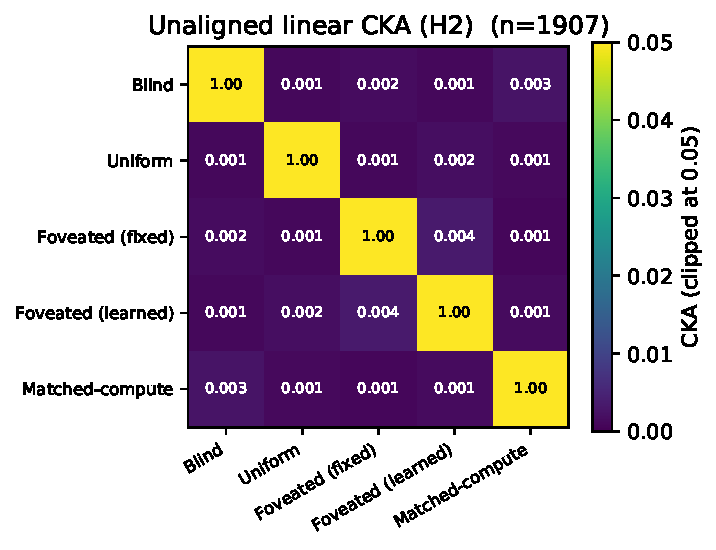
\includegraphics[width=\linewidth]{fig/h2_cka_heatmap.pdf}
\end{minipage}\hfill
\begin{minipage}{0.55\linewidth}\centering
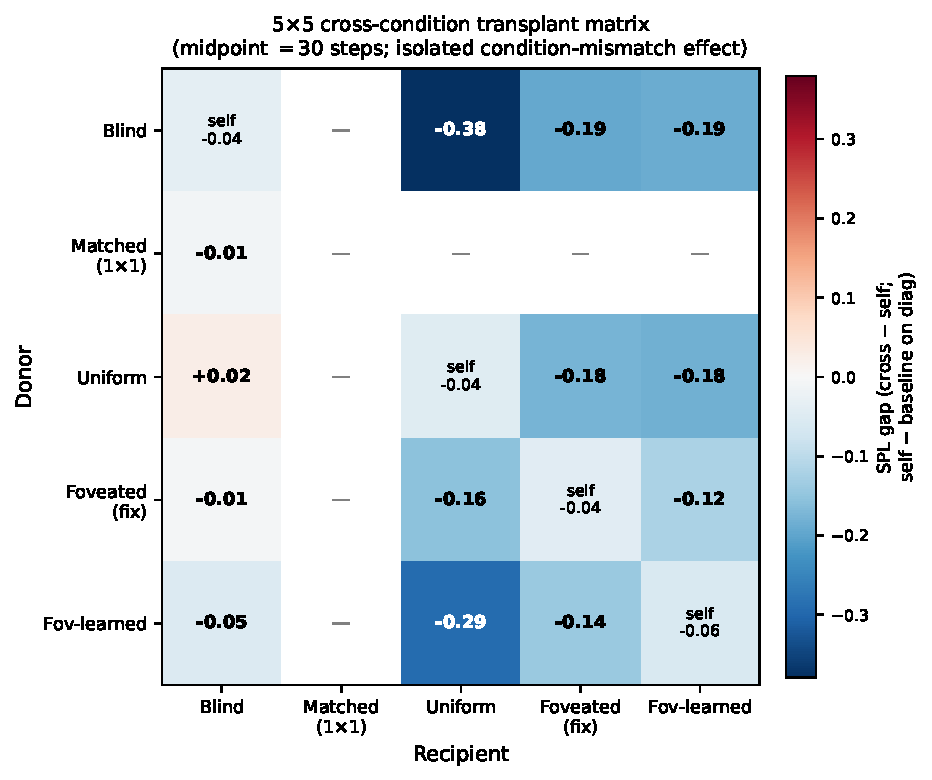
\includegraphics[width=\linewidth]{fig/transplant_5x5.pdf}
\end{minipage}
\caption{H2 convergent evidence, two views. \emph{Left:} Unaligned linear CKA~\citep{kornblith2019cka} between top-layer LSTM hidden states ($n{=}95{,}640$ steps per condition under deterministic-rollout probes); every off-diagonal is below $10^{-4}$. \emph{Right:} 5$\times$5 cross-condition memory-transplant matrix at midpoint $t{=}30$. Cells off-diagonal report cross-transplant SPL minus the recipient's self-transplant SPL (the isolated condition-mismatch component, with rollout-divergence mechanics subtracted); diagonal cells report self-transplant SPL minus baseline (the rollout-divergence noise floor, $\approx-0.04$ to $-0.06$). The matrix is asymmetric: blind$\to$uniform incurs $-0.38$ SPL while uniform$\to$blind is essentially neutral ($+0.02$); foveated-learned$\to$uniform $-0.29$, blind$\to$foveated $-0.19$. \emph{Pairs that are indistinguishable to linear similarity (CKA noise floor) differ markedly under transplant.} Cells with `---' are not yet measured (matched as recipient, jobs in flight). A midpoint-sweep view of three representative pairs across midpoints $\{0, 15, 30, 60, 90\}$ confirming the noise-floor and stability arguments is in Appendix~\ref{app:supp_figs} (Figure~\ref{fig:transplant_sweep_supp}).}
\label{fig:h2}
\end{figure}

\begin{table}[!htbp]
\centering
\small
\caption{Probe-transfer GPS $R^2$ on deterministic-rollout hidden states: train on row condition, test on column. Self-accuracy diagonal is $0.89$--$0.99$; every cross-condition transfer is catastrophically negative ($R^2 \ll -800$, often $\ll -10^4$), reflecting that a probe trained on one condition's hidden-state geometry does not just degrade on another --- it predicts off-manifold values.}
\label{tab:transfer}
\begin{tabular}{lccccc}
\toprule
Train $\backslash$ Test & Blind & Uniform & Fov-fix & Fov-lrn & Matched-compute \\
\midrule
Blind            & \textbf{$+$0.99} & $-$844    & $-11{,}301$  & $-10{,}731$  & $-55{,}706$ \\
Uniform          & $-1{,}383$       & \textbf{$+$0.90} & $-7{,}046$  & $-3{,}305$   & $-110{,}317$ \\
Fov-fix          & $-2{,}091$       & $-2{,}792$ & \textbf{$+$0.92} & $-1{,}263$  & $-39{,}100$ \\
Fov-lrn          & $-6{,}722$       & $-2{,}423$ & $-6{,}205$  & \textbf{$+$0.89} & $-38{,}842$ \\
Matched-compute  & $-10{,}621$      & $-4{,}832$ & $-4{,}984$  & $-58{,}169$  & \textbf{$+$0.96} \\
\bottomrule
\end{tabular}
\end{table}

\noindent\textbf{Behavioural test (memory transplant)}\quad The most direct test of ``do these representations matter?'' is to paste a donor's mid-episode hidden state into a recipient's policy at step $30$ and let the recipient drive the rest (Figure~\ref{fig:h2}, right). The isolated condition-mismatch cost --- cross-transplant SPL minus recipient's self-transplant SPL --- shows three patterns. \emph{Asymmetry.} Blind$\to$uniform incurs $-0.38$ SPL while uniform$\to$blind is neutral within self-noise; bottleneck-donor states hurt rich-encoder recipients far more than the reverse. \emph{Recipient ranking.} Uniform suffers most from \emph{any} foreign donor (column mean $\sim -0.20$); blind least ($\sim -0.02$ to $-0.05$). Blind tolerates foreign donors; rich-encoder recipients do not. \emph{Order-of-magnitude probe-similarity blind spot.} Pairs that are indistinguishable under linear similarity (CKA $<10^{-4}$ across the board) differ by $0.01$--$0.38$ SPL under transplant. \TODO{4 matched-recipient cells of the $5{\times}5$ are queued; asymmetry will be tested for completeness on landing.}

\emph{Convergent linear-similarity evidence.} Three further measures point to the same ``different format'' conclusion. \emph{Pairwise CKA}~\citep{kornblith2019cka} at the noise floor across all condition pairs (Figure~\ref{fig:h2}, left; within-condition split-half CKA $\approx 1$, so the near-zero off-diagonals are not estimator noise). \emph{Cross-condition probe transfer} (Table~\ref{tab:transfer}) is catastrophically negative in every off-diagonal cell, so a probe trained on one condition's hidden states predicts off-manifold values on another. \emph{1-NN purity}: among $1500{\times}5 = 7500$ pooled top-layer states, every sample's Euclidean nearest neighbour shares its condition (purity $1.000$ vs.\ chance $0.20$); a t-SNE projection (Appendix~\ref{app:supp_figs}) confirms this visually. \TODO{1-NN at larger sample size and under domain shift (MP3D / fov-shifted) is a further-investigate item.}

\emph{Ruling out alternatives.} Probe capacity is not the bottleneck (self-probes succeed everywhere); sample-size asymmetry is ruled out by common-sample truncation; task competence is bunched ($96$--$99\%$), so the divergence is not a skill difference; probe transfer fails symmetrically, ruling out one condition's code simply embedding another's.

\emph{Boundaries.} Our similarity tests are linear or near-linear; non-linear measures could reveal higher-order shared structure. Our five sensors are diverse but not exhaustive; hybrid sensors (sharp fovea + coarse periphery, depth-only) might produce intermediate geometries.


\subsection{Foveation: convergence on H1, divergence on H2 + behaviour}
\label{sec:foveation}

Foveated-fixed and uniform fall in the same rich-encoder pass-through regime on the headline H1 metric (top-layer GPS $R^2$ at chance), but they are not interchangeable on H2 / behavioural / dataset-shift axes (Table~\ref{tab:fov-vs-uni}). The take-away: \emph{within the rich-encoder regime defined by H1, foveation and uniform produce internally distinct representations whose differences only the H2-and-beyond machinery makes visible}.

\begin{table}[!htbp]
\centering
\small
\setlength{\tabcolsep}{6pt}
\caption{Foveation vs.\ uniform at $\sigma_{\max} = 8$ Gaussian blur with the same ResNet-18 encoder. Same on H1, different on H2 / behavioural / generalisation. Sources: Table~\ref{tab:summary}, Figure~\ref{fig:h2}, Figure~\ref{fig:shortcut}, Figure~\ref{fig:encoder_probe}. Data are deterministic-rollout single-seed.}
\label{tab:fov-vs-uni}
\begin{tabular}{lccl}
\toprule
Measure & Foveated (fix) & Uniform & Verdict \\
\midrule
LSTM GPS $R^2$ (Gibson) & $+0.06\pm 0.88$ & $-0.31\pm 0.86$ & both chance, \emph{indistinguishable} \\
Encoder $\to$ GPS $R^2$ & $-0.65\pm 0.28$ & $-0.32\pm 0.08$ & both negative, overlapping \\
LSTM compass $R^2$ (Gibson) & $+0.07\pm 0.69$ & $+0.36\pm 0.23$ & uniform $\sim 5\times$ better\\
LSTM GPS $R^2$ (MP3D, held out) & $+0.35\pm 0.27$ & $-0.36\pm 1.38$ & \textbf{differ by 0.71}\\
Shortcut SPL drop \% & $21\%$ & $41\%$ & \textbf{uniform $2\times$ more brittle}\\
Memory-transplant cost (fov $\to$ uni) & \multicolumn{2}{c}{$-0.10$ SPL beyond self-noise} & \textbf{not interchangeable}\\
Pairwise CKA(fov, uni) & \multicolumn{2}{c}{$< 10^{-4}$} & \textbf{near-orthogonal subspaces}\\
1-NN purity (pooled) & \multicolumn{2}{c}{$1.000$ vs.\ chance $0.20$} & \textbf{linearly separable}\\
\bottomrule
\end{tabular}
\end{table}

Four in-flight experiments target specific predictions of the encoder--memory race within the foveation slot (designs in Appendix~\ref{app:foveation-status}). One result has landed and is pivotal:

\begin{figure}[!htbp]
\centering
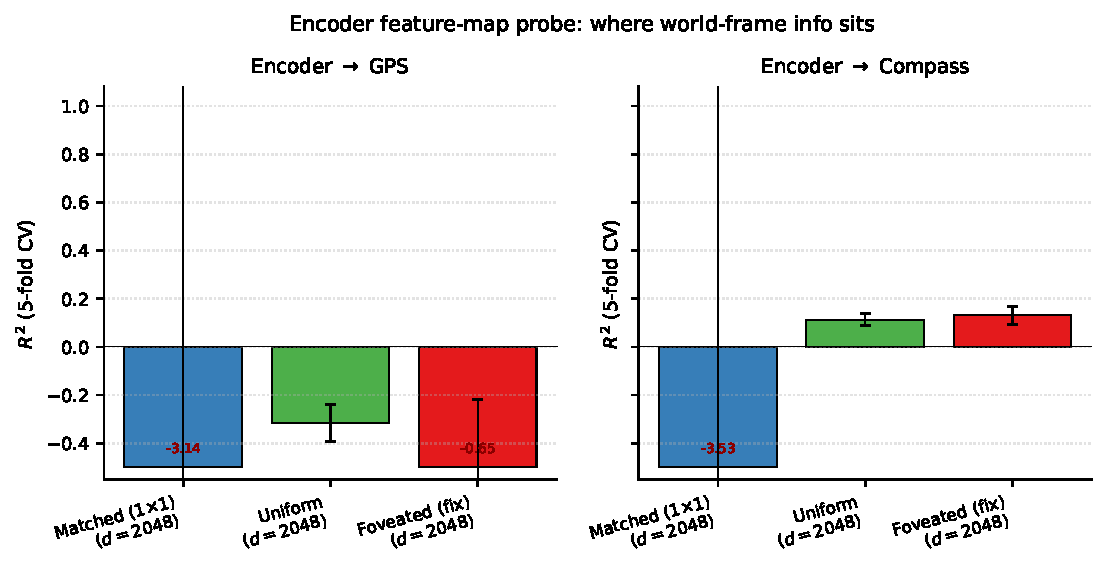
\includegraphics[width=0.92\linewidth]{fig/encoder_feature_probe.pdf}
\caption{Encoder feature-map probe (post ResNet-18, pre-LSTM, 5-fold CV Ridge). Encoder dim $d=2048$ (compressed flatten) for all three sighted conditions. None of the three encoders linearly decode GPS (matched $R^2 = -3.14$, uniform $-0.32$, foveated $-0.65$); the encoder--memory race is therefore not about encoder-level GPS information availability. Compass shows a small positive on uniform / foveated ($+0.11, +0.13$); matched compass is also chance.}
\label{fig:encoder_probe}
\end{figure}

\noindent\textbf{Encoder feature-map probe: where world-frame info actually sits}\quad Probing the visual encoder's output directly (post ResNet-18, pre-LSTM, via forward-hook on the compression layer) gives a striking result: \emph{none of the three sighted encoders linearly decode GPS} (Figure~\ref{fig:encoder_probe}). Compass also fails or is well below ceiling. \emph{This sharpens the H1 mechanism}: the divergence happens inside the LSTM, not at the visual encoder. Bottleneck conditions integrate the GPS-sensor input across time because their visual stream gives the LSTM minimal feature variety to substitute; rich-encoder conditions have richer (though still position-blind) visual features that the LSTM uses instead. The ``LSTM gain'' --- the difference between top-layer LSTM GPS $R^2$ and the encoder's --- is a clean signature: matched gains $+3.9$ R² (LSTM heavily reconstructs from sensor integration), uniform gains $+0.0$ (LSTM fully substitutes visual features for GPS), and foveated gains $+0.7$ (LSTM partially reconstructs --- consistent with foveation supplying \emph{less} navigation-useful visual structure than uniform, so the LSTM cannot rely on visual features alone).

\emph{Provisional conclusion.} Foveation under $\sigma_{\max}=8$ Gaussian blur is \emph{not a copy of uniform}: it converges on H1 but diverges on H2 / behaviour / dataset-shift (Table~\ref{tab:fov-vs-uni}). The encoder feature-map probe further shows the encoder discards linear GPS regardless of condition, so \emph{whatever foveation does differently from uniform, it does it inside the LSTM in subspaces invisible to a linear-GPS probe}. The four in-flight experiments (Appendix~\ref{app:foveation-status}) test \emph{what} that ``something different'' is. F3 log-polar in particular has a falsifiable prediction: log-polar's $\sim 2{\times}2$ encoder spatial output should produce LSTM GPS $R^2 \geq 0.3$ (between matched's $+0.78$ and uniform's $\approx 0$); if instead it matches uniform, the encoder-spatial-output mechanism would need reframing.


\subsection{Probe-readable vs.\ policy-used memory: a $2{\times}2$ dissociation}
\label{sec:dissociation}

H1 (§\ref{sec:h1}) measures what is \emph{readable} from the recurrent state. The shortcut-discovery experiment measures what the policy actually \emph{relies on}: in paired same-scene/different-goal episodes ($20$ scenes $\times$ $10$ pairs), the second-episode SPL drop under persistent vs.\ reset memory indexes how tightly the policy couples actions to integrated recurrent memory (blind loses $52\%$, uniform $41\%$, foveated $21\%$, matched $18\%$, foveated-learned $15\%$). Plotting probe-readable GPS against this behavioural reliance reveals a $2{\times}2$ pattern (Figure~\ref{fig:shortcut}) with two opposite anomalies. Matched-compute has a linear top-layer GPS code yet its policy weights it less than the probe predicts; uniform has no linear GPS but relies heavily on memory --- plausibly via non-spatial scene-history features. ``Probe-readable'' and ``policy-relied-on'' can therefore dissociate in either direction.

\begin{figure}[!htbp]
\centering
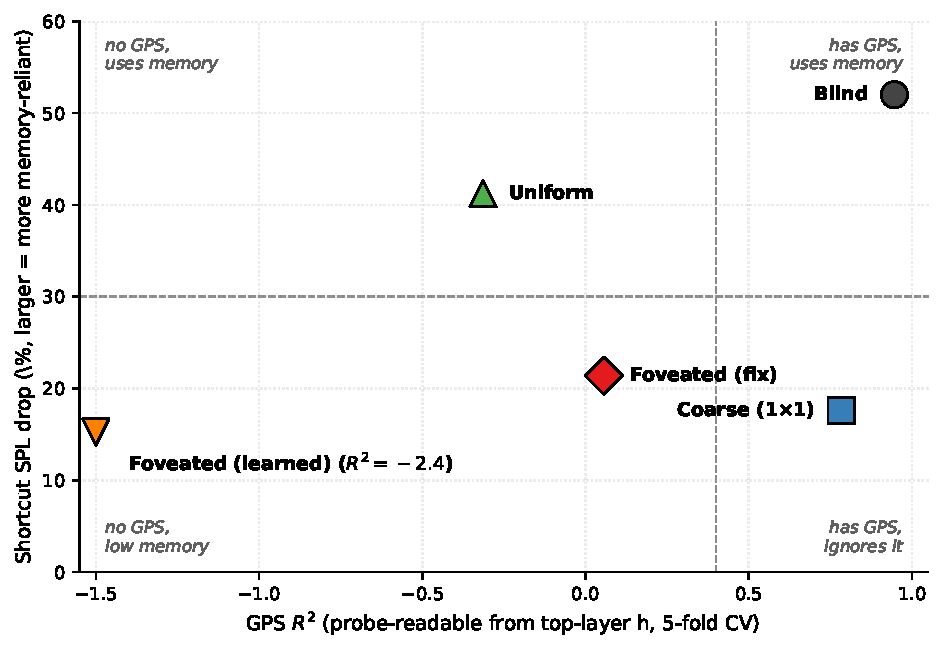
\includegraphics[width=0.62\linewidth]{fig/shortcut_scatter.pdf}
\caption{Probe-readable GPS (H1) vs.\ behavioural memory reliance (shortcut). The five conditions occupy four corners of a $2{\times}2$: blind ``has GPS, uses memory'' (consistent with H1); foveated-fixed and foveated-learned ``no linear GPS, low memory reliance'' (also consistent with H1); \textbf{matched} and \textbf{uniform} are the two off-diagonal anomalies. Fov-learned's $R^2 = -2.43$ is clipped at $-1.5$.}
\label{fig:shortcut}
\end{figure}

A trajectory-level look at \emph{how} persistent-memory failures manifest sharpens the dissociation (Figure~\ref{fig:shortcut_paired_traj}). Quantifying across all same-floor paired-episode failures, only uniform's persistent agent ends up closer to the previous-episode goal than to the new one (Table~\ref{tab:lock-onto-old}, margin $+1.83$m, $n{=}46$); blind's persistent runs end nearer the new goal but never reach it (margin $-0.38$m). This pattern is consistent with the $2{\times}2$: \emph{uniform's memory acts as a visual / scene-history anchor} that locks the agent in place, whereas \emph{blind's GPS code interferes via a different channel} (the recurrent state mis-reporting current position to the policy's goal-direction integrator). The single-seed nature of these claims is a limitation; multi-seed replication is in flight.

\begin{figure}[!htbp]
\centering
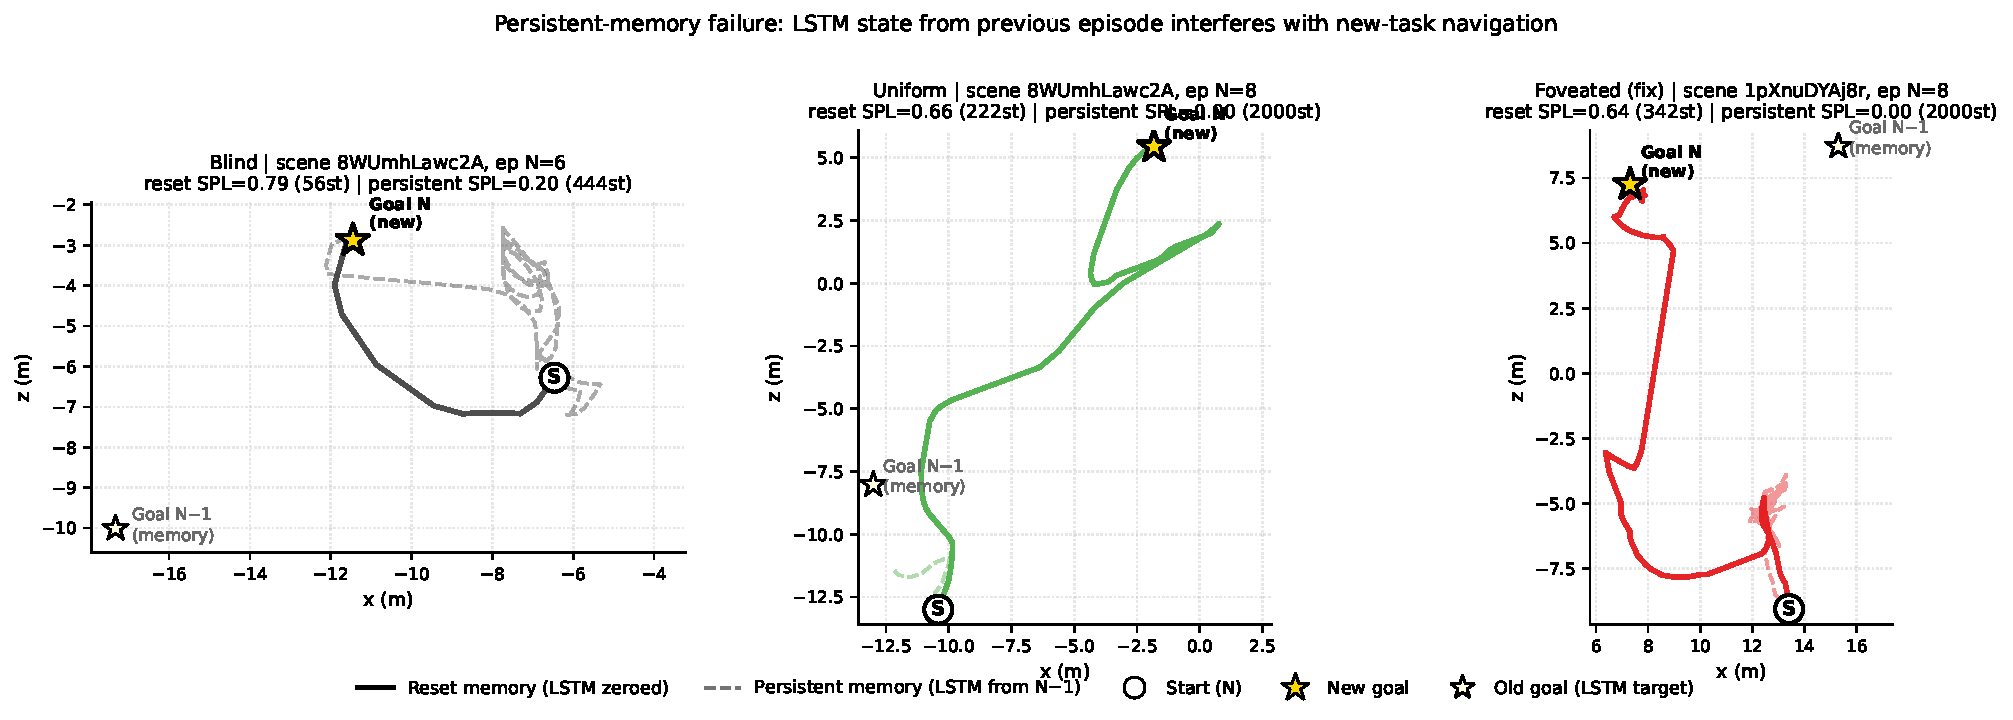
\includegraphics[width=\linewidth]{fig/shortcut_paired_traj.pdf}
\caption{Three persistent-memory failure modes (one paired-episode case per condition). \emph{Blind}: persistent agent attempts the new goal, loops, gives up at $443$ steps. \emph{Uniform}: persistent agent stays \emph{at} the old-goal location for the full $2000$-step cap. \emph{Foveated}: persistent agent loops chaotically in a region distant from both goals.}
\label{fig:shortcut_paired_traj}
\end{figure}

\begin{table}[!htbp]
\centering
\small
\caption{Where the persistent agent ends up (same-floor paired-episode failures: reset SPL $>0.5$, persistent SPL $<0.2$, persistent steps $\geq 30$, $|\Delta y_\text{goal}| < 0.5$m). Only uniform's failures cluster nearer the previous-episode goal.}
\label{tab:lock-onto-old}
\begin{tabular}{lcccccc}
\toprule
Condition & $n$ & avg dist $\to$ old (m) & avg dist $\to$ new (m) & margin (m) & Closer to & Reading \\
\midrule
Blind            & 27 & 7.48 & 7.10 & $-0.38$ & new & tries new, fails \\
Matched          & 35 & 6.29 & 5.72 & $-0.57$ & new & tries new, fails \\
\textbf{Uniform} & 46 & \textbf{6.45} & 8.28 & $\mathbf{+1.83}$ & \textbf{old} & locks onto old \\
Foveated (fix)   & 16 & 7.01 & 6.42 & $-0.59$ & new & wanders \\
Fov-learned      &  5 & 3.89 & 6.19 & $+2.30$ & old & ($n{=}5$, low confidence) \\
\bottomrule
\end{tabular}
\end{table}


\subsection{Gaze location (H3, in progress)}
\label{sec:h3}

H3 asks whether gaze \emph{location} acts as a second representational-content axis within the rich-encoder regime. Our minimal learned-gaze module (deterministic sigmoid MLP, slow updates per 128-step segment) freezes at $(0.49, 0.62)$ with per-dimension std $\leq 2.5\times 10^{-4}$ after 250M frames; anti-collapse regularisers restore variance only at task-cost (Appendix~\ref{app:gaze_diversity}). The collapse is not evidence about active gaze in general --- the decoder is minimal by design --- but it provides an empirical anchor for the gaze-location test: a foveated-shifted control with gaze hardcoded at $(0.49, 0.62)$ instead of $(0.5, 0.5)$, identical to foveated-fixed in every other respect, isolates static gaze location from the optimisation-path interaction that produced the collapsed gaze. Training is in progress at submission.


\subsection{Boundaries}
\label{sec:boundaries}

Three probes that do \emph{not} discriminate define the boundary of our claims. Coarse occupancy decodes above chance everywhere; metric $20{\times}20$ occupancy fails everywhere (consistent with~\citep{ramakrishnan2025space} that high-resolution metric layout needs non-linear probes); the ego-frame goal vector is at chance everywhere because PointGoal supplies it as a per-step input. Population coding (Appendix~\ref{app:supp_figs}) sharpens H1 in a direction we did not expect: rich-encoder conditions have a few units with \emph{higher} peak spatial information than blind, but those peaked units do not decode GPS --- suggesting they encode features merely correlated with position (visual landmarks, trajectory phase). Blind's broader, lower-peak distribution carries the actual linear position code.


\FloatBarrier
\section{Discussion}
\label{sec:discussion}

\subsection{Two orthogonal axes: sensor structure and gaze location}

Our findings unify under a candidate account we call the \emph{encoder--memory race}: top-layer linear GPS encoding in the LSTM is \emph{maintained} when the encoder hands the LSTM minimal spatial-feature variety per step (blind, matched-compute), and \emph{overwritten} when richer visual features substitute (uniform, foveated, foveated-learned). The encoder feature-map probe (§\ref{sec:foveation}) confirms that no sighted encoder linearly re-derives GPS, so the H1 race is not encoder-vs-LSTM at the position-information level; it is at whether the LSTM has visual variety enough to substitute for integrating its Layer-0 GPS-sensor signal across time. H2 (§\ref{sec:h2}) cuts orthogonally: \emph{what} the LSTM encodes lives in distinct linear subspaces across conditions, and the difference matters for behaviour (cross-condition memory transplants drop SPL beyond transplant-mechanics noise; the $5\times5$ matrix is asymmetric). H3 (§\ref{sec:h3}) asks whether, within the rich-encoder pass-through regime, gaze location is a second content axis; the foveated-shifted causal control is in training. We present the unifying account as a candidate, not a proven mechanism: a direct causal test (e.g.\ ablating the visual stream mid-rollout) is left for follow-up.

\subsection{Biological precedent: sensor structure shapes hippocampal representation}
\label{sec:bio}

The principle that sensor structure constrains spatial-memory format is not one we propose; biological evidence for it predates ours by decades. Our contribution is to isolate the principle in a controlled silicon model where the encoder, memory, policy, training distribution and reward are held fixed and only the visual sensor varies. Three threads of animal-navigation research are particularly close to the three findings.

\emph{H1 (sensor bottleneck $\to$ memory takes over).} Congenitally blind humans show enhanced occipital--hippocampal coupling during spatial tasks~\citep{kupers2014blind}, consistent with hippocampus carrying more navigational load when the visual stream is absent. Rodent grid-cell periodicity collapses under prolonged darkness while the animal still navigates~\citep{chen2016grid}, indicating spatial behaviour can be sustained when the visual landmark stream is removed. Both are biological analogs of our blind / matched-compute regime, where the LSTM --- deprived of rich visual variety per step --- retains a linear top-layer GPS code that the rich-encoder conditions overwrite.

\emph{H2 (different sensors $\to$ different spatial codes).} The primate vs.\ rodent contrast in hippocampal cell types --- view-cells dominant in primates, place-cells dominant in rodents --- has been attributed in part to the foveated-with-saccades vs.\ near-panoramic visual sampling regime each species uses~\citep{rolls2024why}. Cross-modality remapping in echolocating bats, where the same neurons recode under vision vs.\ echolocation~\citep{geva2016remapping}, demonstrates that sensor modality alters the linear subspace of hippocampal coding. Both parallel our H2 finding: the same task with different visual structure yields linearly separable LSTM subspaces (CKA $<10^{-4}$, probe-transfer collapse, asymmetric memory transplant).

\emph{H3 (gaze location modulates memory encoding).} In primates, hippocampal theta is gated by saccades, and the reliability of this saccade-gated signal predicts memory encoding success~\citep{jutras2013saccades,tas2016overt}. Where the eye points is therefore not memory-neutral. Whether the analogous prediction holds for an LSTM gaze module is what §\ref{sec:h3} is testing (foveated-shifted causal control in training).

We treat these as convergent (not conclusive) evidence. Convergence across systems --- and across silicon vs.\ neural --- is suggestive of a sensor--memory coupling principle more general than any single architecture, but it does not show that the mechanisms are the same. Our experiments isolate the principle in a controlled, single-architecture setting; biological work establishes that the principle exists in animals at all. The two are complementary; neither is decisive alone.

\subsection{Why this, not alternative accounts}

Four alternative explanations are ruled out: skill difference (success bunched 93--99\%), probe capacity (DtG decodes everywhere), sample-size or stochastic-sampling artefacts (Appendix~\ref{app:probing-details}), and linear-probe artefact (memory transplant reproduces the ordering outside the probe framework; MLP probe shows the divergence is specific to \emph{linear} top-layer decodability, which is what the linear DD-PPO action head reads). Full rebuttals in Appendix~\ref{app:alt-accounts}.

\subsection{Implications for ML practice and architectural scope}

Within the recurrent PointNav setting we study, three implications follow. (i)~\emph{Encoder capacity correlates inversely with linear, top-layer, policy-accessible LSTM spatial encoding}; if causal (Appendix~\ref{app:scaling} tests this), it is also a practical training-time lever for inducing cognitive-map-like internal representations. (ii)~\emph{``More pixels'' is not the right lens}: the linear top-layer GPS code is non-monotonic in raw pixel count (uniform $256^2$ lacks it; matched $48^2$ with $1{\times}1$ feature map has a strong one). The encoder feature-map probe shows neither encoder linearly preserves GPS, so the mechanism is not encoder position retention; we attribute the pattern to encoder spatial-feature variety per step, with the scaling sweep and log-polar control needed to confirm. (iii)~\emph{Gaze (H3 pending):} within the rich-encoder regime, we predict shifting the static gaze location alters what the LSTM encodes; the foveated-shifted causal control is in training (§\ref{sec:h3}).

\noindent\textbf{Beyond the recurrent setting (untested)}\quad The three implications are established only in our LSTM setting. Transformer-based embodied agents build their internal state by accumulating information via learned attention, structurally similar to our gaze location in the sense that it selects which observation content is read into the representation; H3 therefore suggests a testable prediction for transformer navigators (strong constraints on attended tokens $\to$ content-level dissociations like ours) which we do not verify here. The sensor-structure axis (H1, H2) is a claim specifically about RL recurrent navigation agents under partial observability; whether equivalent effects arise in supervised visual learners, non-visual modalities, or multimodal systems is an open question.

\subsection{Limitations}
\label{sec:limitations}

(i)~\emph{Intermediate checkpoint for foveated-fixed:} all foveated-fixed analyses use ckpt.36 at $\sim$174M, the last checkpoint before the silent-corruption window (Appendix~\ref{app:training-stability}); the other four conditions use the final converged checkpoint. (ii)~\emph{Minimal learned-gaze architecture.} Our learned-gaze module is a deterministic sigmoid MLP with slow-gaze rollout updates, chosen for computational compatibility with DD-PPO rollouts and simplicity as a controlled variable, not as a competitive active-gaze model. Its collapse under pure task supervision is specific to this architecture (and so far to a single seed; multi-seed replication is in progress); richer gaze mechanisms (stochastic gaze with entropy bonus, information-seeking intrinsic reward, attention-based token selection) would need separate investigation. We therefore do not claim that implicit task pressure cannot produce active gaze in general; we claim only that our minimal decoder collapsed, and we use the collapsed-gaze position as an empirical starting point for the gaze-location test (foveated-shifted control, §\ref{sec:h3}) --- a test whose logic does not depend on the gaze decoder working. (iii)~\emph{Cross-heading probe:} the proposal included a cross-heading generalisation probe (train on heading $A$, test on opposite heading). Our implementation returned ``insufficient samples'' sentinels at our probe sizes and does not appear in our results. (iv)~\emph{Foveation model:} Gaussian blur with quadratic falloff is a simplification; log-polar or multi-scale pyramid models may behave differently. A log-polar control (F3) and a $\sigma_{\max}\in\{2,4,12,20\}$ strength sweep (F1--F4) are in training at submission and will populate §\ref{sec:foveation} and Appendix~\ref{app:foveation-status}. (v)~\emph{Linear probes only:} non-linear probes might reveal structure Ridge regression misses, particularly for occupancy maps. (vi)~\emph{Architecture scope:} we use a recurrent (LSTM) backbone to remain comparable with the emergent-map literature we build on. The core claims (sensor structure and gaze location as representational-content axes) should hold for transformer-based navigation agents whose internal state is built by learned attention, but directly verifying this requires re-running the five-condition ablation on a transformer backbone and is left for future work; see §\ref{sec:discussion} for the specific predictions.


\section{Conclusion}

We ran a controlled five-condition ablation isolating the effect of visual-input structure on the recurrent representations learned by an otherwise-identical DD-PPO navigation agent. Three findings emerge.

\emph{(1)~Encoder--memory race (H1).} Top-layer LSTM GPS encoding is \emph{temporally stable} when the encoder hands the LSTM minimal spatial-feature variety per step (blind, matched-compute), and \emph{transient} when richer visual features substitute (uniform, foveated, foveated-learned). The encoder feature-map probe shows no sighted encoder linearly decodes GPS, so the H1 mechanism lives inside the LSTM, not at the encoder. H1 is most precisely a claim about \emph{linear, top-layer, late-episode} GPS encoding --- what the linear DD-PPO action head can read.

\emph{(2)~Condition-specific representational format (H2).} Even where rich-encoder LSTMs are spatially pass-through, their hidden-state subspaces are linearly separable to single-nearest-neighbour granularity (CKA $<10^{-4}$, probe transfer $\ll -800$, 1-NN purity $1.000$). The $5\times5$ memory-transplant matrix is asymmetric: bottleneck donor states hurt rich-encoder recipients far more than the reverse. Whatever non-spatial task-relevant features each LSTM carries, it carries them in its own linear subspace.

\emph{(3)~Gaze location (H3, pending) and a having--vs.--using dissociation.} Whether gaze location is a second content axis \emph{within} the rich-encoder regime is in training (foveated-shifted control). Independently of that pending test, plotting probe-readable GPS against behavioural memory reliance reveals a 2$\times$2 dissociation: matched has linear GPS but ignores it; uniform has no linear GPS but heavily uses memory. Both anomalies rest on single-seed runs and we mark them as candidate dissociations pending multi-seed replication.

The pattern parallels three threads of animal-navigation research --- enhanced hippocampal coupling in congenitally blind humans, the disruption of rodent grid-cell firing in darkness with navigation nonetheless preserved, and cross-modality hippocampal remapping in bats. We use these as analogy only: the convergent direction across systems is suggestive of a sensor--memory coupling principle, but our experiments do not test architectures other than LSTM, so we do not claim the principle is architecture-independent. Open questions: (i)~whether the encoder-bottleneck ordering extends to finer-grained resolution sweeps (Appendix~\ref{app:scaling}); (ii)~whether H3 stands on the clean causal test; (iii)~whether transformer-based navigation agents reproduce the encoder--memory race; (iv)~whether equivalent effects shape representations in non-navigation embodied tasks; (v)~multi-seed replication of all five conditions to bound seed-to-seed variability of the H1 numbers.


\bibliographystyle{plainnat}
\bibliography{literature}

\newpage
\input{checklist}

\newpage
\appendix

\section{Probing protocol details}
\label{app:probing-details}

\noindent\textbf{Sampling protocol}\quad An earlier draft used stochastic (policy-distribution) action selection at probe time. Conditions with higher action-entropy under their trained stochastic policies sampled the STOP action early with $\sim 0.25$ per-step probability, producing $\sim 4$-step rollouts and target variance two orders of magnitude below the episodic range. The resulting probe $R^2$ values were trivially high across all conditions (any predictor fits a near-constant target). This confounded cross-condition comparisons; we switched to the deterministic (argmax) protocol used here and elsewhere in our pipeline. All paper results use the deterministic protocol.

\emph{Length-matching ablation.} Under deterministic rollouts, episode lengths span $\sim$100--400 mean steps depending on condition. We use 5-fold episode-level CV to keep splits balanced per scene rather than length-matching across conditions. \TODO{A controlled length-matching ablation (truncate every condition to a common length) is left for follow-up; we expect it to leave the H1 ordering unchanged because the bottleneck conditions decode at high $R^2$ even at the smallest sub-sample, but have not verified.}

\emph{Cross-heading probe.} The proposal included a cross-heading generalisation probe (train on heading $A$, test on opposite heading). Our implementation returned ``insufficient samples'' sentinels at our probe sizes; not in our results.

\section{Probing details (Layer 0 sensor branch and MLP probe)}
\label{app:probe-details}

\emph{LSTM Layer 0 sensor branch.} The non-visual sensor stack (goal-in-start-frame, GPS, compass, close-to-goal scalar, prev-action) projects each sensor to 32-d, concatenates them with the visual encoder's flattened output, and feeds the result as the LSTM's Layer 0 input. The GPS embedding therefore enters the LSTM via this concatenation; this explains why Figure~\ref{fig:h1_mega}c shows linearly-decodable GPS at Layer 0 even for conditions whose visual encoder discards GPS entirely.

\emph{MLP probe details.} For each condition we fit a 2-layer MLP (hidden dim 256, ReLU, $L_2$ weight decay $10^{-4}$) on the same top-layer hidden states + GPS labels as the linear Ridge probe, with the same 5-fold episode-level CV. Top-layer recovery: foveated $R^2 = 0.51$, foveated-learned $0.73$, uniform $0.55$ (vs.\ Ridge's chance R²). The MLP probe alone cannot disentangle ``non-linear position code'' from ``MLP regressing through position-correlated features (wall distance, scene identifiers, episode-phase markers)''; the resolution scaling sweep (Appendix~\ref{app:scaling}) tests this more directly by varying input resolution at fixed encoder stack.

\section{Alternative-account rebuttals (full)}
\label{app:alt-accounts}

\emph{Task-competence differences.} All conditions solve PointGoal at $93$--$99\%$ success (Table~\ref{tab:summary}); the encoded-content gap cannot be attributed to navigation skill.

\emph{Probe-capacity / probe-fitting artefacts.} DtG decodes robustly across all five conditions ($R^2 \geq 0.81$), demonstrating Ridge has the capacity to fit high-$R^2$ scalars when the hidden state contains them. Hewitt--Liang label-permutation selectivity is high where GPS is high (blind, matched) and at chance where GPS is at chance --- the latter follows from real and control probes facing the same near-zero target-information ceiling. The chance-level rich-encoder $R^2$ is therefore a hidden-state property, not a probe artefact.

\emph{Sample-size / trajectory-distribution artefacts.} CV $\sigma$ spans come from the same 500-episode pool with $\sim 100$--$400$-step rollouts under identical deterministic evaluation; the protocol confound that haunted an earlier draft is documented and retired in Appendix~\ref{app:probing-details}.

\emph{Linear-probe artefacts.} Two complementary checks. \emph{(a)~Behavioural:} the memory-transplant intervention goes outside the probe framework and reproduces the bottleneck-vs-pass-through ordering; the $5\times 5$ matrix's asymmetry adds a structure no linear-similarity measure can read. \emph{(b)~Non-linear probe:} a 2-layer MLP recovers $R^2 \in [0.51, 0.73]$ from rich-encoder top-layer states (Appendix~\ref{app:probe-details}). The bottleneck-vs-pass-through divergence is therefore not about whether \emph{any} probe can recover position; it is specifically about whether a \emph{linear} top-layer probe can. Since the DD-PPO action head is a linear projection from $\mathbf{h}_2$, the linear metric is what the policy itself can use, so H1 maps onto policy-accessible encoding regardless of how the MLP interpretation resolves.


\section{Supplementary visualisations}
\label{app:supp_figs}

\begin{figure}[h]
\centering
\begin{minipage}{0.52\linewidth}\centering
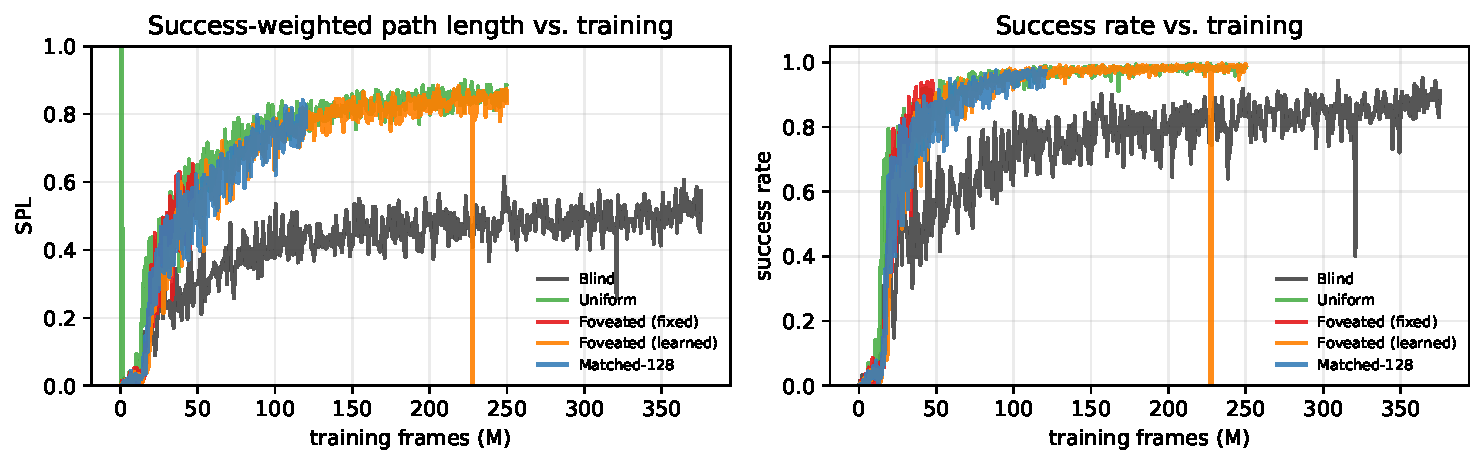
\includegraphics[width=\linewidth]{fig/training_curves.pdf}\\
{\footnotesize (a) Training curves (TensorBoard event-file scalars). All four sighted conditions converge to SPL $0.82$--$0.85$ and success $>97\%$ by $\sim$100M frames; blind converges to SPL $\sim$0.50 over a longer horizon. The glitch at frame~$\approx 228$M (fov-learned) is a resume-boundary artefact in the scalar log.}
\end{minipage}\hfill
\begin{minipage}{0.44\linewidth}\centering
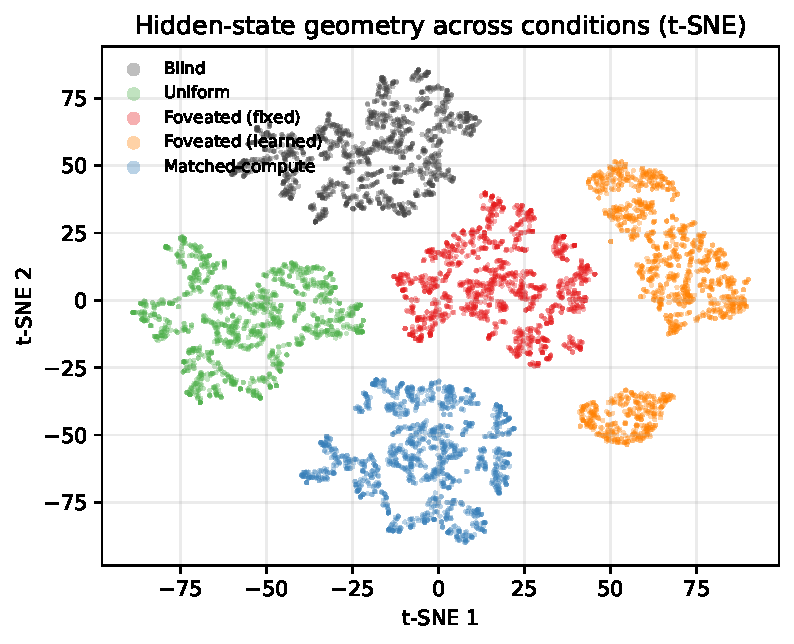
\includegraphics[width=\linewidth]{fig/h2_hidden_embedding_tsne.pdf}\\
{\footnotesize (b) t-SNE projection of top-layer LSTM hidden states (deterministic-rollout probes), pooled across all five conditions (perplexity 30). The five conditions occupy non-overlapping regions of the 2-D embedding --- a visual confirmation of the near-zero CKA result (§\ref{sec:h2}).}
\end{minipage}
\caption{Supplementary visualisations referenced from the main text.}
\label{fig:supp_figs}
\end{figure}

\begin{figure}[h]
\centering
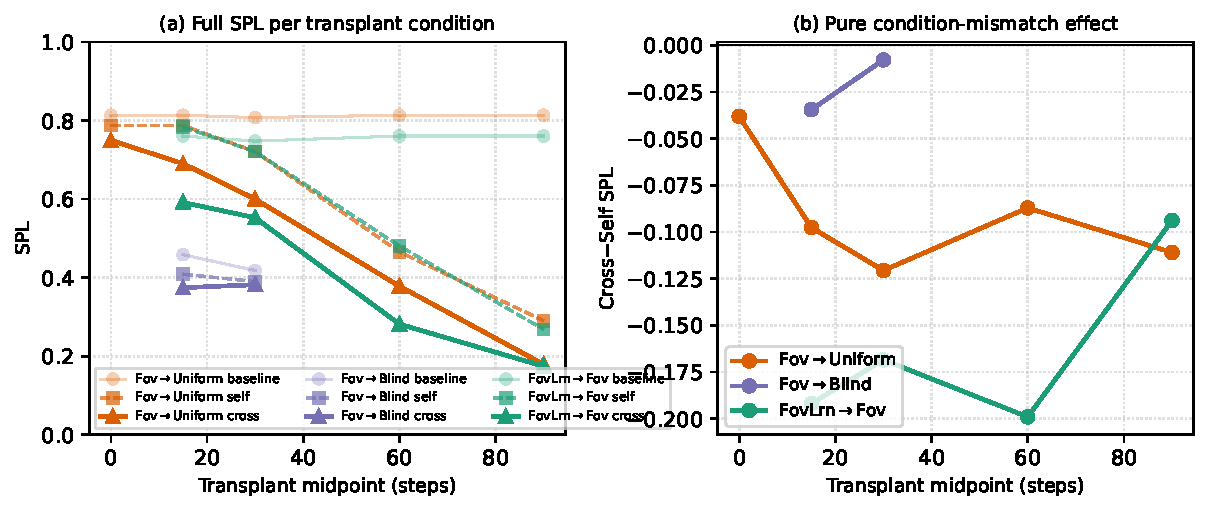
\includegraphics[width=0.95\linewidth]{fig/transplant_sweep.pdf}
\caption{Memory-transplant midpoint sweep on three representative donor$\to$recipient pairs (foveated$\to$uniform, foveated$\to$blind, foveated-learned$\to$foveated) across midpoints $\{0, 15, 30, 60, 90\}$ time-steps ($n{=}100$--$150$ episodes/cell). The full $5{\times}5$ matrix in Figure~\ref{fig:h2} (right) is at midpoint $t{=}30$; this supplementary figure shows that the cross-self gap is roughly stable for $t \geq 15$ and that the $t{=}0$ self-/cross- baseline collapses to a protocol-noise floor (so the diagonal in Figure~\ref{fig:h2} is correctly read as ``rollout-divergence noise'' rather than ``condition-mismatch noise''). Foveated-learned$\to$foveated incurs $-0.17$ SPL on average across $t \geq 15$, foveated$\to$uniform $-0.10$, foveated$\to$blind $-0.02$, consistent with the asymmetry pattern in the full matrix.}
\label{fig:transplant_sweep_supp}
\end{figure}

\begin{figure}[h]
\centering
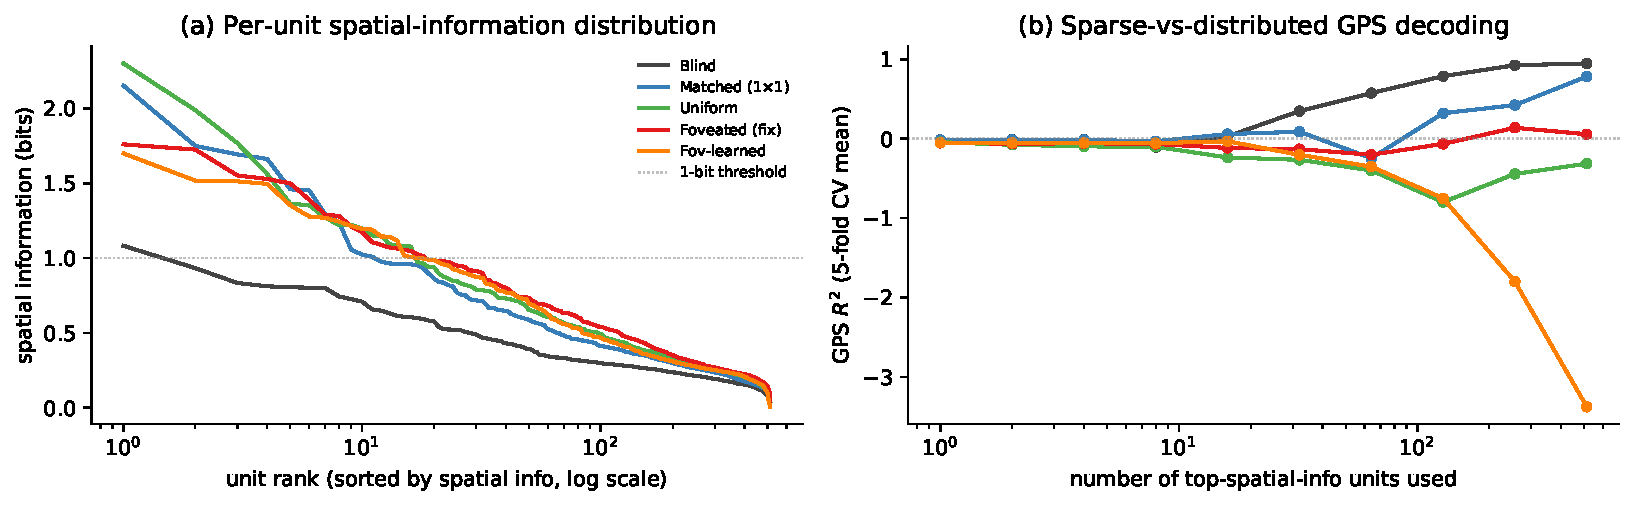
\includegraphics[width=0.95\linewidth]{fig/population_coding_summary.pdf}
\caption{Population coding analysis (referenced from §\ref{sec:boundaries}). \emph{(a)}~Per-unit spatial-information distribution: each curve is one condition's units sorted by spatial information (descending), x-axis log scale. Counter-intuitively, rich-encoder conditions (uniform / foveated / fov-learned) have a few more peaked spatially-tuned units (max $\approx 2$ bits) than bottleneck conditions; blind has the flattest distribution (max $\approx 1$ bit, no unit reaches the dashed 1-bit threshold). \emph{(b)}~Sparse-vs-distributed GPS decoding: probe $R^2$ when only the top-$k$ spatial-info units are used as features. Blind reaches $R^2 \approx 1.0$ at $k=512$; matched climbs to $R^2 \approx 0.5$; rich-encoder networks fail to decode GPS at any $k$ even though their top units carry higher per-unit spatial information. The combined picture: \emph{higher per-unit spatial information $\neq$ position readout}. Rich-encoder peaked units appear to encode features correlated with position (e.g.\ visual landmarks, trajectory phase) rather than position itself.}
\label{fig:supp_pop_coding}
\end{figure}

\begin{figure}[h]
\centering
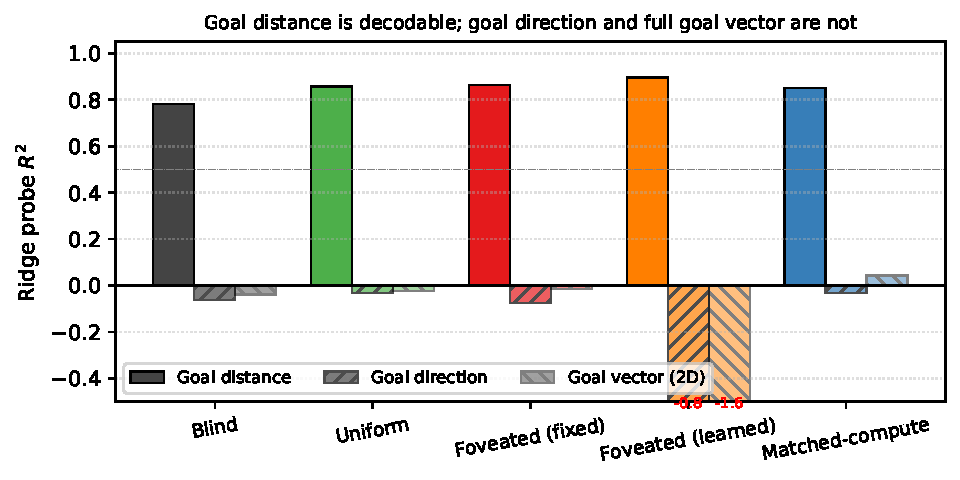
\includegraphics[width=0.7\linewidth]{fig/goal_vector_probe.pdf}
\caption{Goal-vector probe $R^2$ (referenced from §\ref{sec:boundaries}). Goal \emph{distance} (DtG) decodes strongly across all conditions ($R^2 \in [0.81, 0.90]$, validating probe machinery); goal \emph{direction} and the full ego-frame goal vector are at chance or negative everywhere. PointGoal provides the goal vector as a per-step input, so the policy has no incentive to re-encode it.}
\label{fig:supp_goal_vec}
\end{figure}

\begin{figure}[h]
\centering
\begin{minipage}{0.48\linewidth}\centering
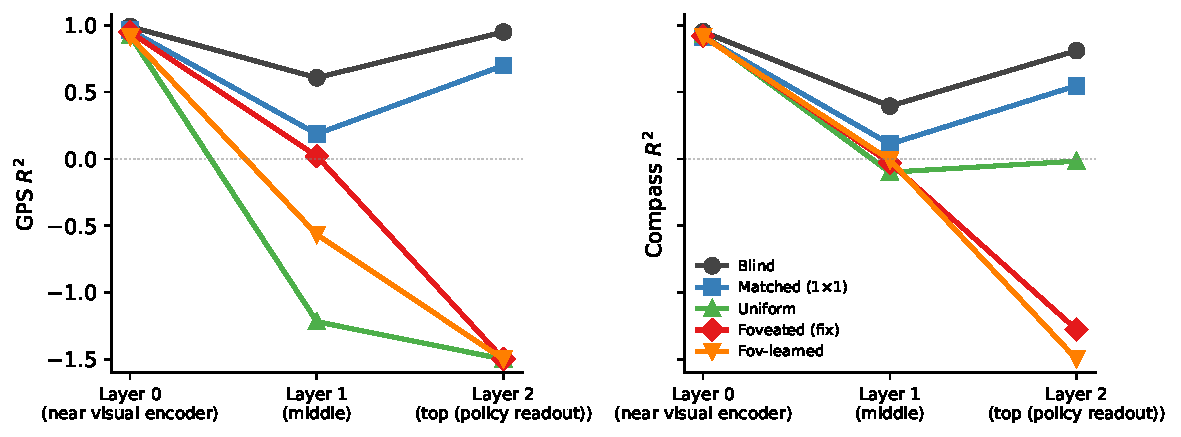
\includegraphics[width=\linewidth]{fig/layerwise_decay.pdf}\\
{\footnotesize (a) Per-LSTM-layer GPS / compass probe $R^2$ across all three layers, all five conditions (single train/test fit; the 5-fold CV mean reported in Table~\ref{tab:summary} matches qualitatively but with different magnitudes for rich-encoder conditions). Compass tells the same story as GPS at smaller magnitude.}
\end{minipage}\hfill
\begin{minipage}{0.48\linewidth}\centering
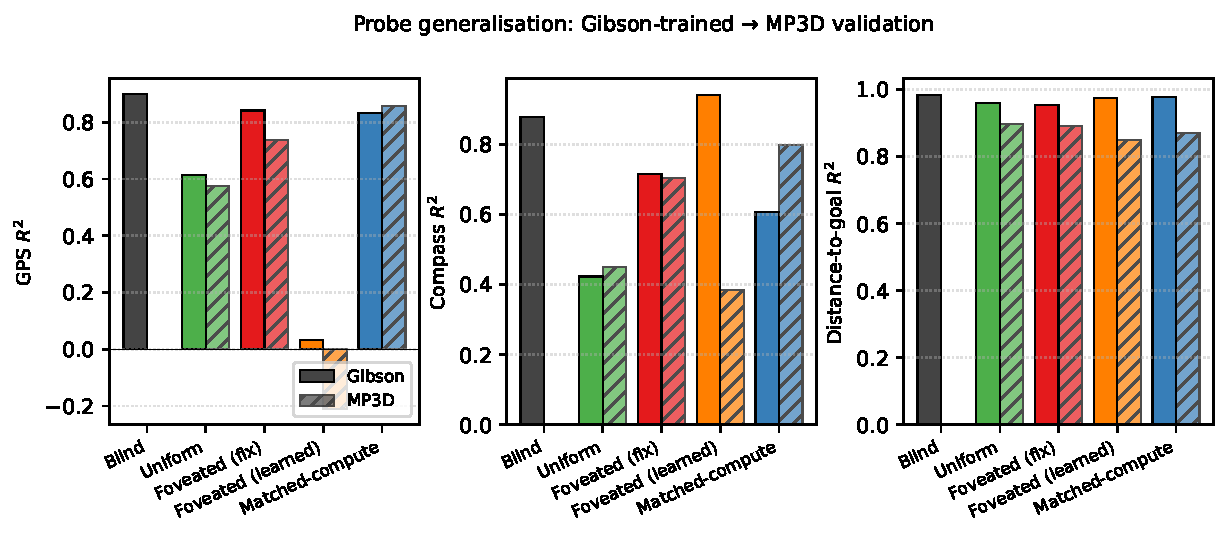
\includegraphics[width=\linewidth]{fig/mp3d_generalization.pdf}\\
{\footnotesize (b) Companion to Figure~\ref{fig:h1_mega}d (which uses 5-fold CV mean): single train/test fit on the same checkpoints; the qualitative bottleneck-vs-pass-through partition is the same.}
\end{minipage}
\caption{Per-layer and MP3D companion figures (referenced from §\ref{sec:h1}).}
\label{fig:supp_layerwise_mp3d}
\end{figure}


\section{Gaze-Diversity Auxiliary Loss (H3 Ablation)}
\label{app:gaze_diversity}

\emph{Motivation.} In the first foveated-learned training run the gaze decoder collapsed (per-dimension std $\approx 5\times 10^{-4}$). We attribute this to two mechanisms: (i)~once the sigmoid output saturates, its derivative $\sigma'(x)\to 0$ attenuates gradient signal; (ii)~consistent-gaze views yield more predictable visual features, so the reward-gradient path has no explicit incentive for variety.

\emph{Target-variance hinge.} We add $\mathcal{L}_\text{div} = \lambda \cdot \text{relu}(\sigma^2_\text{target} - \text{Var}_\text{batch}[g])$ where $g \in [0,1]^2$, $\text{Var}_\text{batch}$ averaged over the two gaze dimensions, $\sigma^2_\text{target}=0.01$ (std $\approx 0.1$), $\lambda = 0.01$. The hinge disappears once variance exceeds the target. We also evaluated an un-capped $-\lambda\cdot\text{Var}[g]$ variant as a negative control.

\emph{Pilot 1 (uncapped, job 2840256).} After 10\,M frames, gaze variance exceeded that of a uniform distribution over $[0,1]^2$ (std $[0.43, 0.42]$ vs.\ theoretical max $0.289$): gaze was essentially random. Task performance collapsed: SPL plateaued at $0.05$, running-mean metrics transitioned to NaN at $\sim 8$\,M frames. The uncapped regulariser destroyed the consistent-foveation signal the policy needs.

\emph{Pilot 2 (hinge, job 2842288).} Gaze converged to an extreme corner of image space: mean $(0.001, 0.998)$ with std $[0.020, 0.023]$ --- well below the target std of $0.1$ and therefore with the hinge active throughout. Task SPL plateaued at $0.05$ as in pilot 1. The policy apparently found the minimum-task-cost gaze that partially satisfies the diversity pressure: a sigmoid saturated at one corner, producing a constant image-corner view.

\emph{Interpretation.} Both pilots argue that in our deterministic sigmoid-MLP gaze architecture with slow-gaze rollouts, gaze collapse is a pre-requisite for task learning rather than an accident. Task signal alone does not spontaneously produce informative fixation, and an exogenous anti-collapse regulariser moves gaze toward whatever region reduces regulariser loss fastest, which is generically \emph{not} the task-useful region. A genuine H3 test likely requires (i)~a stochastic gaze location with entropy bonus, so diversity is sampled at rollout time rather than enforced on a deterministic output; or (ii)~a task-aligned intrinsic reward (e.g., information gain about goal-relative position); or (iii)~an architectural change separating gaze generation from visual-feature extraction (e.g., attention-based gaze).


\section{Training Stability: Silent Weight Corruption in DD-PPO}
\label{app:training-stability}

During an initial foveated training run we observed a failure mode that did not manifest as a crash but as slow, silent corruption of the learned weights. After $\approx$170M frames of stable progress (reward $\approx 10$, SPL $\approx 0.83$), one mini-batch on one DDP worker produced a NaN gradient. Because \verb|torch.nn.utils.clip_grad_norm_| does not sanitise non-finite gradients---the global norm becomes NaN, the clip coefficient becomes NaN, and \verb|grad *= NaN| remains NaN---the subsequent \verb|optimizer.step()| wrote NaN into every parameter. DDP all-reduce propagated the corruption across workers. The training loop did not raise: it continued for 2.5 days with reward$=$NaN and SPL$=0$ until \verb|torch.multinomial| finally rejected the NaN probability tensor. All checkpoints saved during this window were unrecoverable (90 of 97 parameter tensors entirely NaN).

To isolate the origin of the NaN gradient we re-ran training from the last clean checkpoint with \verb|torch.autograd.set_detect_anomaly(True)| and per-module forward-output hooks. The anomaly traceback pinned the failure to \verb|MseLossBackward0|, i.e.\ the backward pass of the value-head loss $\tfrac{1}{2}(V(s) - R)^2$; rare return-vs-value discrepancies overflowed float32 in the squaring step, producing non-finite gradients downstream.

Our mitigation is a minimally invasive patch to \verb|PPO.before_step| that zeroes any non-finite gradient element before clipping. A bad mini-batch becomes a no-op update rather than a catastrophic one. The patch is a no-op on clean training paths. Across the five conditions reported here, no NaN events were observed during full training after deployment, and all final checkpoints contain only finite weights. We reported the underlying issue upstream (habitat-lab issue \#2226) with a minimal reproduction and a proposed native fix.


\section{Foveation experiments: status and design}
\label{app:foveation-status}

This appendix details the four controlled foveation experiments referenced from §\ref{sec:foveation}. All four are submitted; numbers will populate §\ref{sec:foveation} in revision as they land.

\begin{table}[h]
\centering
\small
\caption{Foveation experiment status (submission time).}
\label{tab:fov-status}
\begin{tabular}{lll}
\toprule
Experiment & Tests & Status \\
\midrule
F1--F4 strength sweep ($\sigma_{\max} \in \{2, 4, 12, 20\}$) & encoder--memory race as continuous lever & in training \\
F3 log-polar foveation                                       & spatial-sampling vs.\ blur bottleneck    & in training \\
Encoder feature-map probe (matched / uniform / foveated)     & where position information is held       & \textbf{landed; see §\ref{sec:foveation}} \\
Foveated-shifted (gaze $(0.49, 0.62)$)                       & gaze-location axis (links to H3)         & in training \\
\bottomrule
\end{tabular}
\end{table}

\emph{Foveation strength sweep (F1--F4).} We train four additional foveated agents at $\sigma_{\max} \in \{2, 4, 12, 20\}$ alongside the existing $\sigma_{\max} = 8$, holding gaze location, encoder stack, training budget, and training pool fixed. Expected signature: at low $\sigma_{\max}$ the foveated agent should look like uniform; at high $\sigma_{\max}$ it should approach matched-compute. The $R^2$ vs.\ $\sigma_{\max}$ curve directly tests the encoder--memory race as a continuous lever rather than a binary one.

\emph{Spatial sampling vs.\ blur (F3 log-polar).} Gaussian blur removes high-frequency content but preserves spatial layout: a $\sigma_{\max}=8$ foveated image still feeds the encoder $256{\times}256$ pixels, so the ResNet-18 stack still produces an $8{\times}8$ spatial feature map. A log-polar foveation~\citep{strasburger2011peripheral,rosenholtz2016peripheral} resamples with a non-uniform retinal grid (e.g.\ $64{\times}64$): the encoder spatial output drops to $\sim 2{\times}2$, much closer to matched's $1{\times}1$ than to uniform's $8{\times}8$. This isolates the variable our sharpened H1 mechanism identifies as the trigger: \emph{spatial-feature variety in the encoder output}. Falsifiable prediction (written before result available): log-polar should produce LSTM GPS $R^2 \geq 0.3$, between matched's $+0.78$ and uniform's $\approx 0$, with corresponding behavioural shifts. If instead log-polar matches uniform, the encoder-spatial-output-dimensionality mechanism is wrong. F3 in training (\textasciitilde 14M / 250M frames at submission, ETA 2--3 days).

\emph{Foveated-shifted (gaze location).} Training a foveated agent with hardcoded static gaze at $(0.49, 0.62)$ matches foveated-learned's collapsed gaze location while removing the learned-gaze module from the optimisation path. If foveated-shifted does \emph{not} reproduce foveated-learned's specific behaviours (Gibson--MP3D compass swing, transplant ranking), those behaviours can be attributed to the optimisation-path interaction rather than to gaze location alone. Links to H3 (§\ref{sec:h3}).

\emph{Why disclose this rather than wait.} Each experiment has a falsifiable signature; we disclose the designs openly so (i)~the submission is honest about what foveation-specific evidence already exists vs.\ what is in flight, and (ii)~the reader can identify which incoming result would change the paper's interpretation.


\section{Encoder-capacity scaling sweep}
\label{app:scaling}

\TODO{The scaling sweep trains matched-compute variants at input
resolutions $\{32, 48, 64, 96, 128, 192\}$ alongside the existing blind
(no encoder) and uniform $256{\times}256$ anchors. Probe results on the
trained checkpoints will populate Figure~\ref{fig:scaling} and this
appendix section. Hypothesis: GPS probe $R^2$ decreases monotonically
with input resolution, from $R^2 \approx 0.95$ at no-encoder to
$R^2 \approx 0$ at $256{\times}256$, crossing into the pass-through
regime between $48$ and $128$ pixels.}

\begin{figure}[h]
\centering
\fbox{\rule{0pt}{4cm}\rule{0.8\linewidth}{0pt}}
\caption{Encoder-capacity scaling curve. \TODO{Pending data.} x-axis: input resolution in pixels; y-axis: GPS and compass probe $R^2$ (5-fold CV, mean$\pm\sigma$).}
\label{fig:scaling}
\end{figure}


\end{document}
